
	\chapter{Conception}
	
	\section{Introduction}
	The aim of this chapter is  to study and design the features already determined in the previous phase of analysis and specification of requirements. For that, it is divided into two parts. The first part is dedicated to the exhibition of the choice of conception method as well as the architecture of the system to be developed. The second part presents the conception of the application with a set of diagrams.
	\section{Modeling Language}
		A modeling language is used to describe a system, a standard or methodology, general or domain-specific and / or context based on its components and relationships.
	There are several modeling languages, the best known are UML and Merise.
	\\
	\\
	In our project we chose UML as Modeling language, for two main reasons: 
	\begin{itemize}
	\item To obtain a very high level modeling independent of the language and environments
	\item Document a project. 
	\end{itemize}
	
	\section{Global Conception}
	In this section, we highlight the architecture of our application, we starting  with physical architecture and the logical architecture.
	
	\clearpage
	\newpage
	\subsection{Physical Architecture}
	It is primordial to designing any computer system to choose the model architecture that will be adequate to ensure proper functioning, performance, the reuse and reliable interconnection of this system with others. We opt for this purpose for the physical architecture described in the figure below.
	\begin{figure}[h]
		\centering
		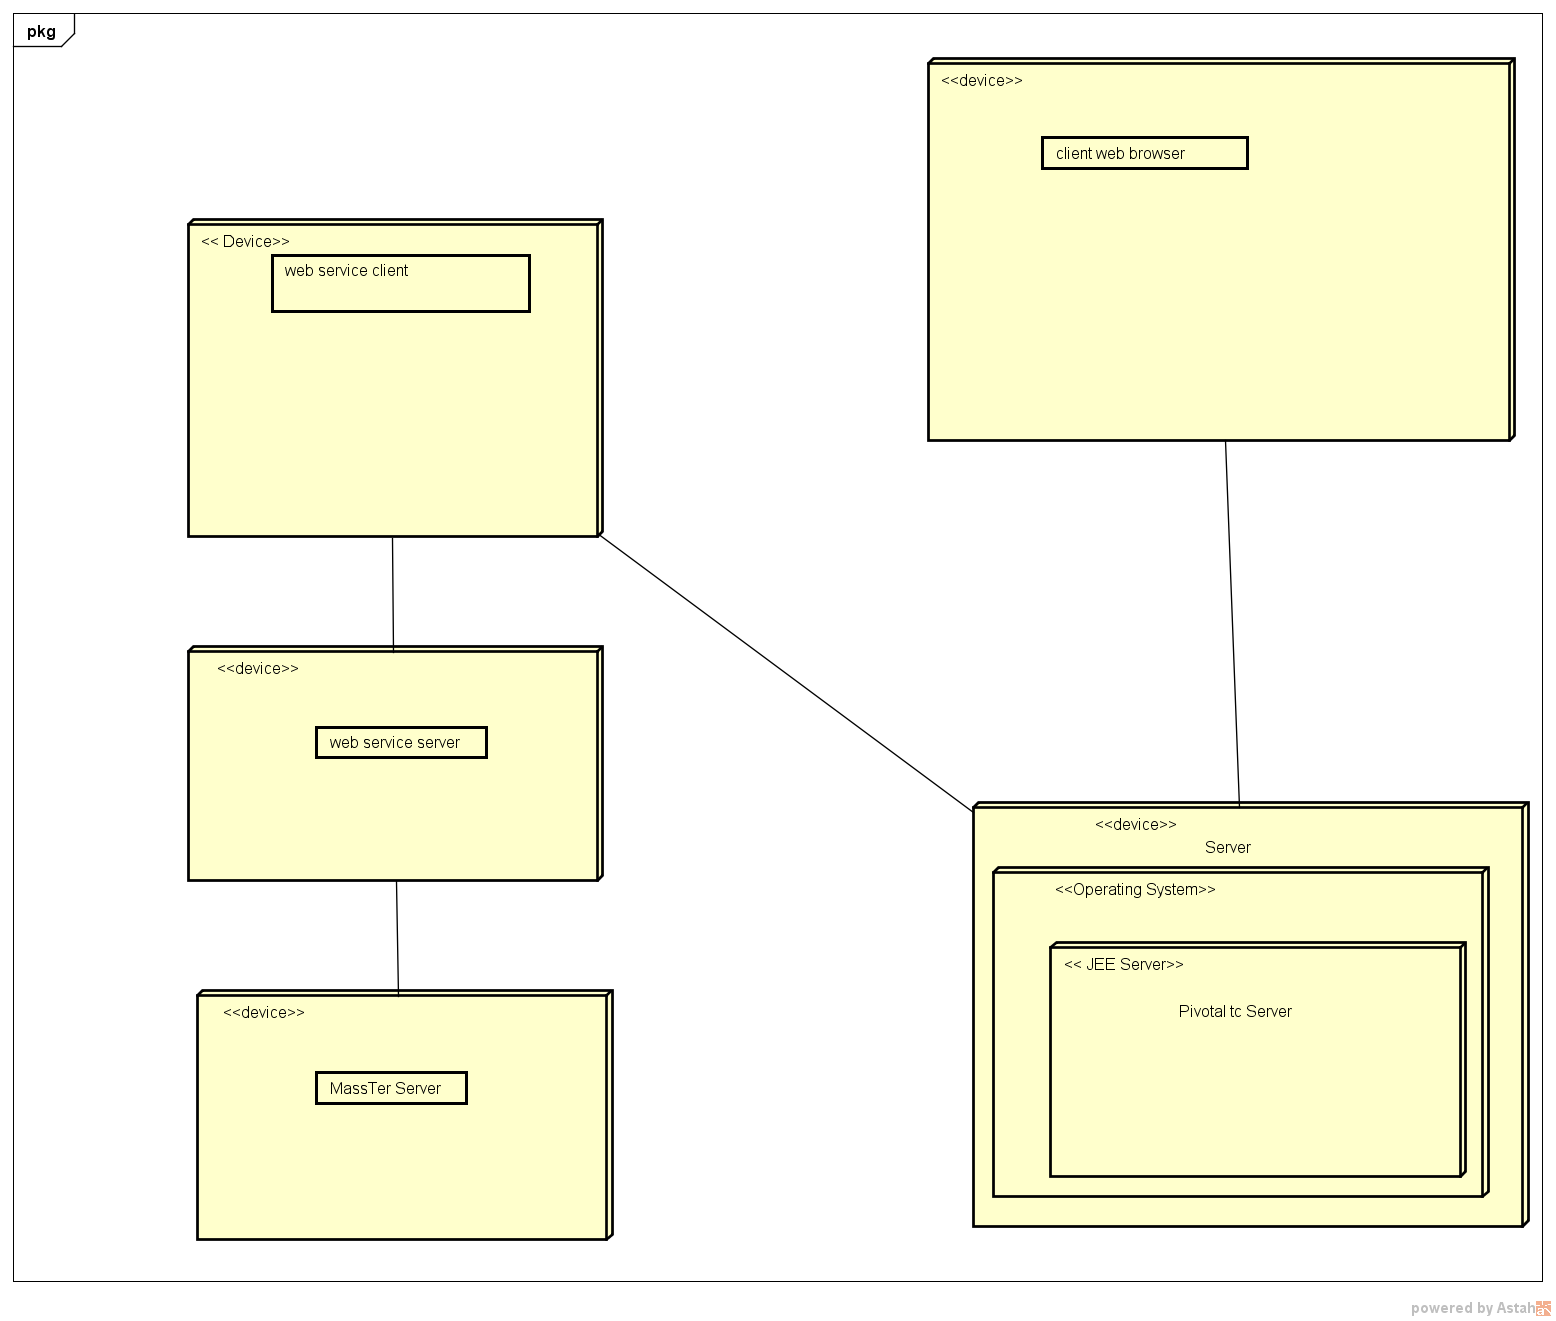
\includegraphics[width=16.5cm,height=12cm]{DeploymentDiagramPhysicalArchitecture.png}
		\caption{Deployment Diagram Physical Architecture}
	\end{figure}  

	\clearpage
    \newpage  
	
	\subsection{Logical Architecture}
 Fig. \ref{logicalArchitecture}	depicts the logical architecture in which different components interact.
\begin{figure}[h]
	\centering
	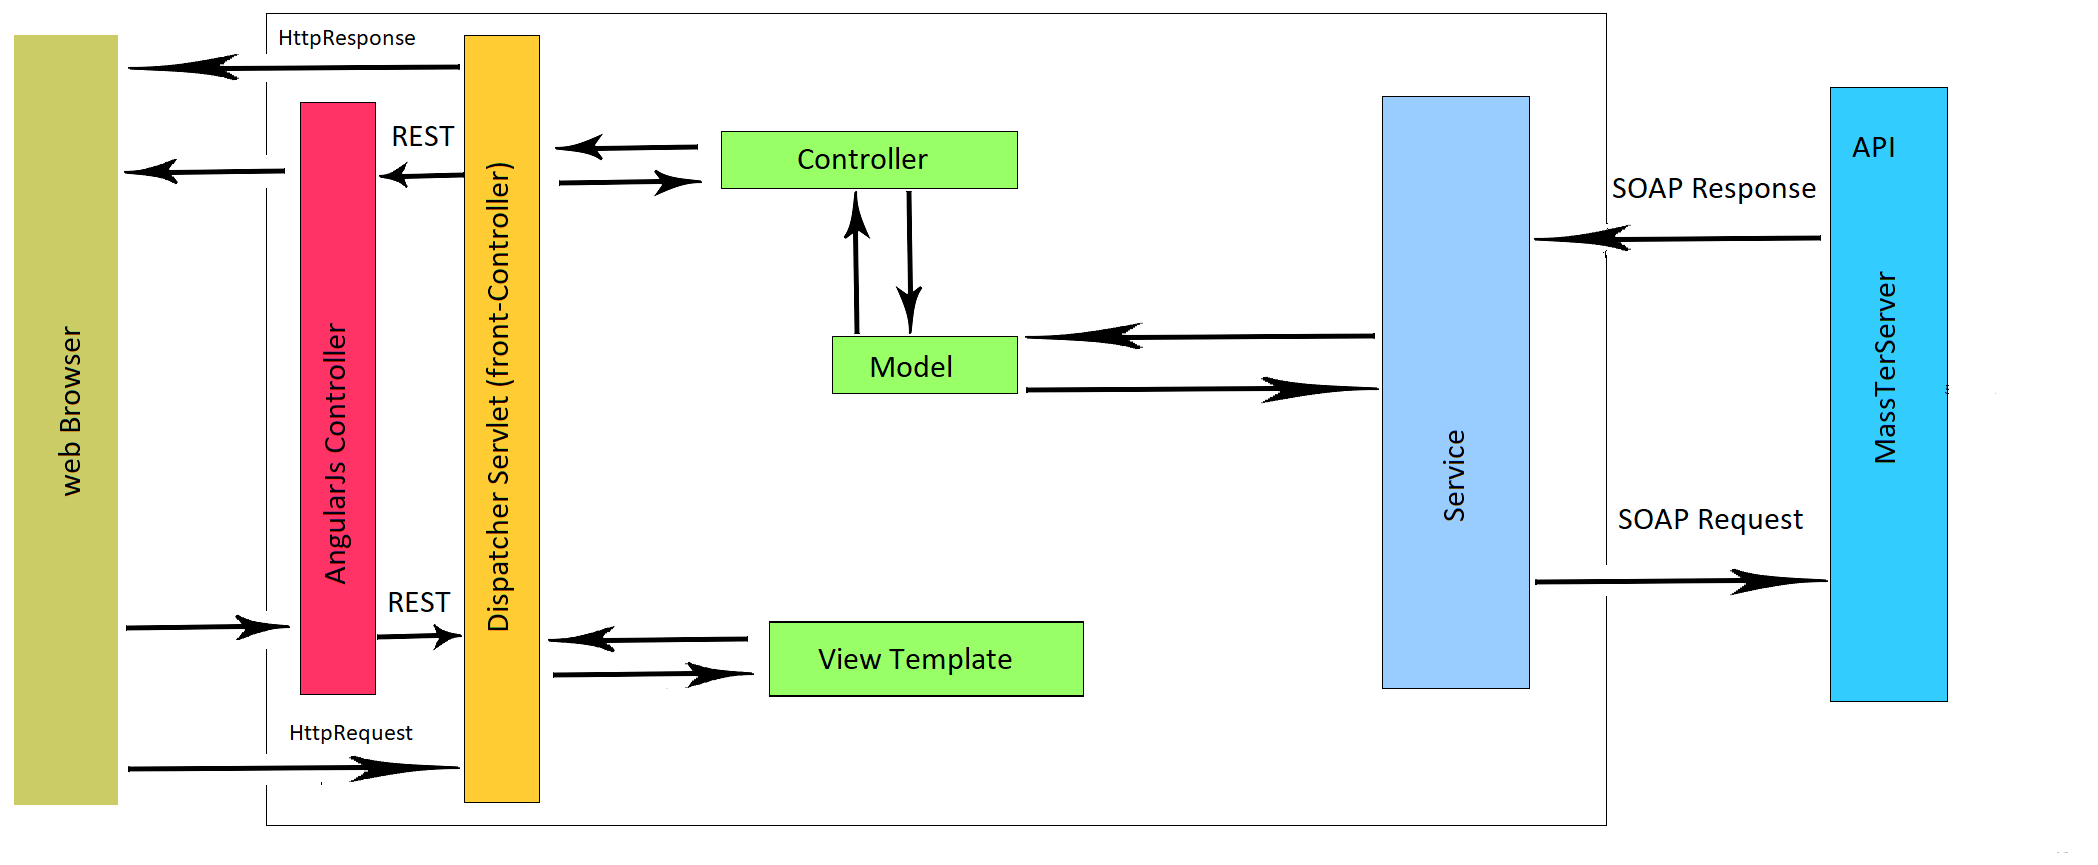
\includegraphics[width=17.5cm,height=9cm]{logicalArchitecture.png}
	\caption{Logical Architecture}
	\label{logicalArchitecture}
\end{figure} 
	
	\subsection{Design Pattern}
		We opt to use the MVC design pattern for the following benefits:
	\begin{itemize}
		\item \textbf{Reliability : }The presentation and business layers are completely separate, so that the business can change without necessarily affecting the presentation, or vice versa.
		\item \textbf{Adaptability : }Any visual representation can be easily integrated.
		\item \textbf{Productivity : }The duration of development is significantly reduced, in allowing parallel work teams.
		\item \textbf{Extensible : } With MVC the code is extensible.
	\end{itemize}

	\clearpage
    \newpage

	\section{Detailed Conception}
	\subsection{Package Diagram}
		\begin{figure}[h]
		\centering
		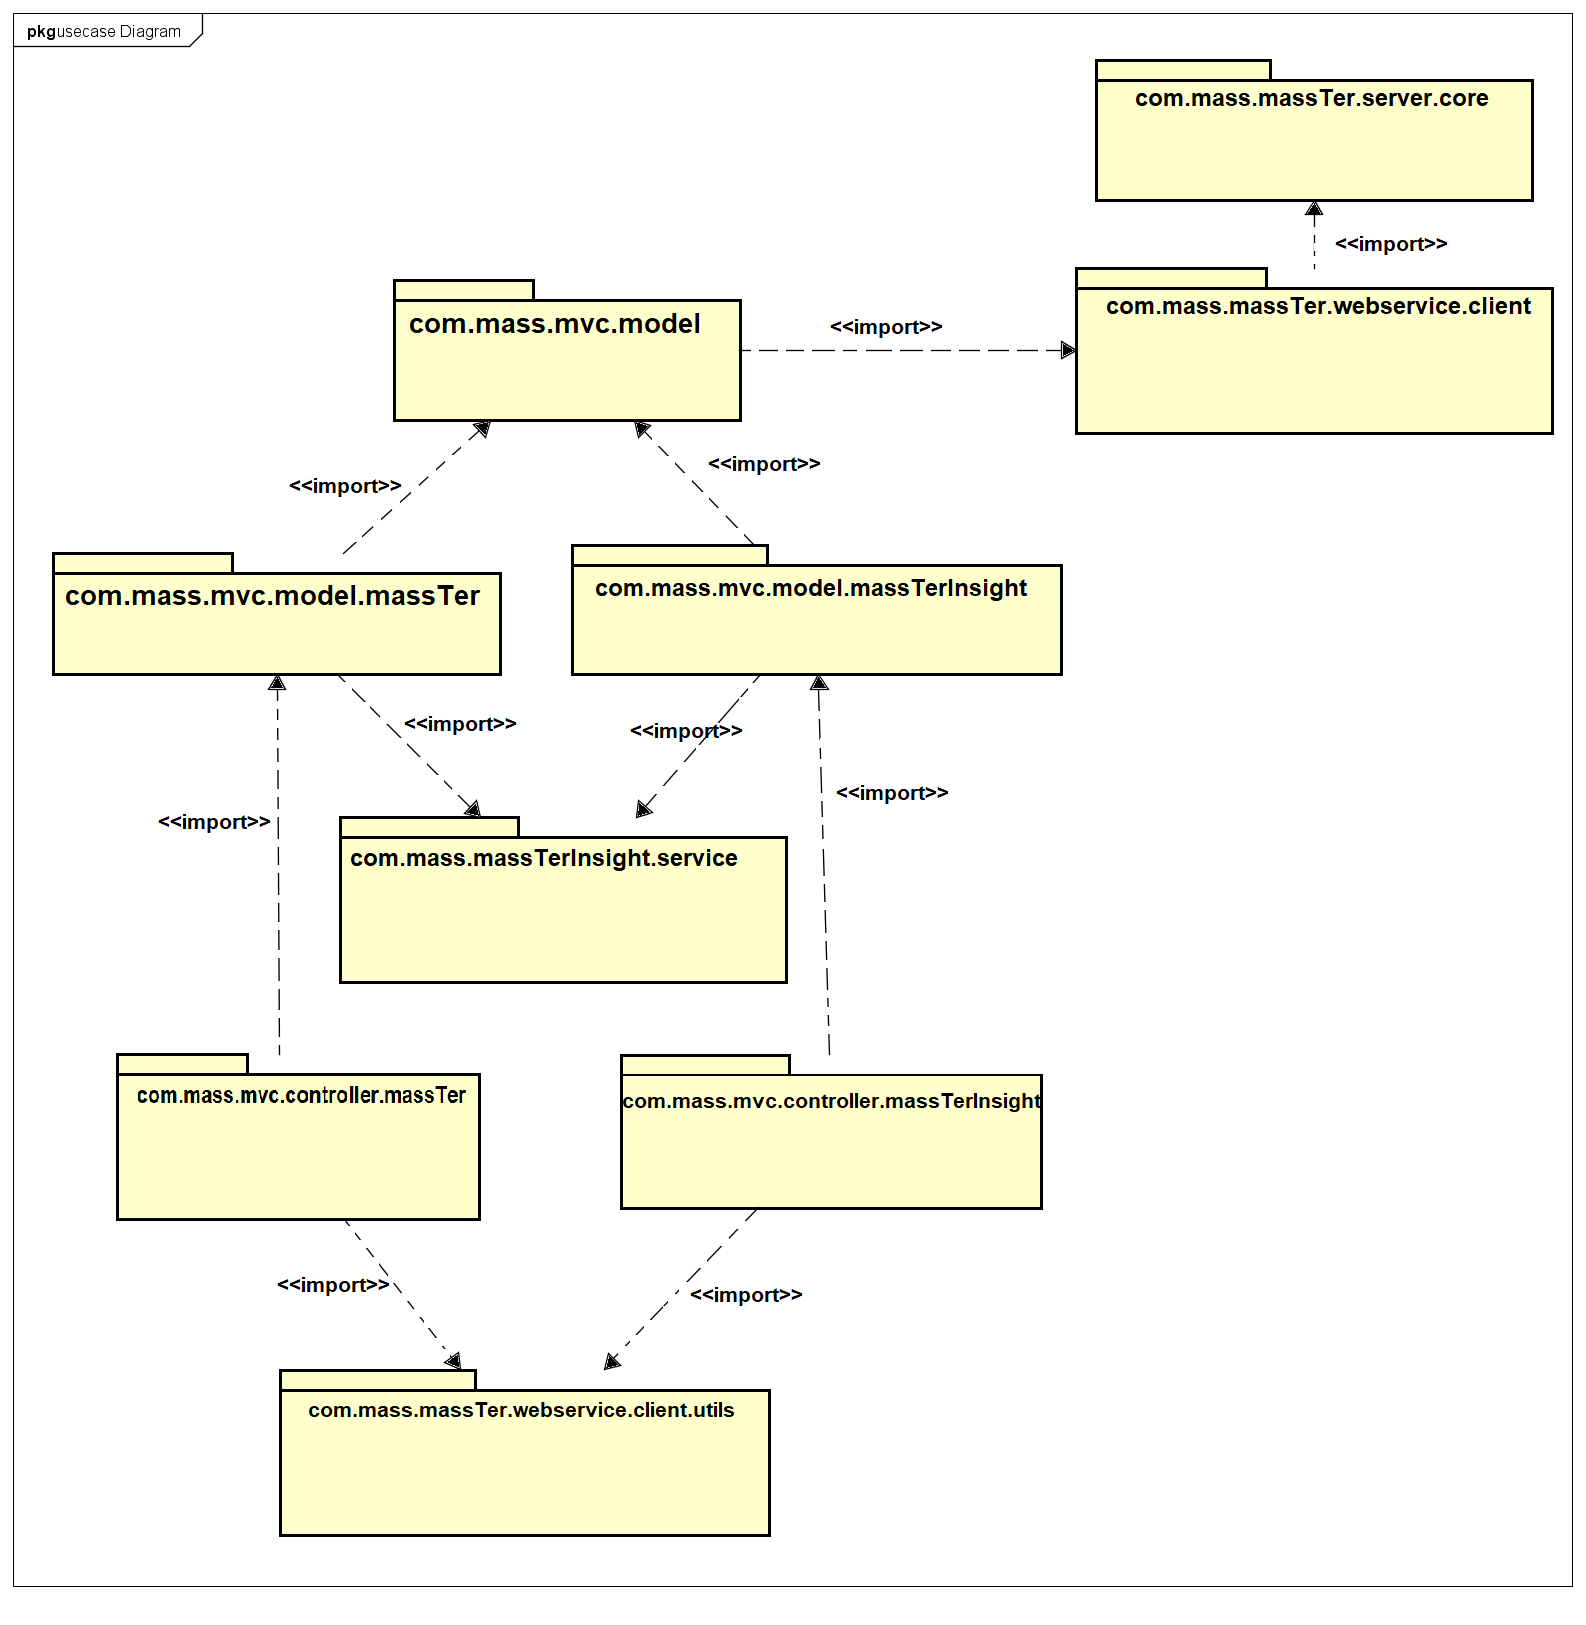
\includegraphics[width=1\textwidth]{packageDiagram.png}
		\caption{package diagram}
	\end{figure}
  
	\pagebreak
	\clearpage
	\newpage
	\subsection{Class Diagram}
			\begin{figure}[h]
		\centering
		\includegraphics[width=17.5cm,height=14cm]{classDiagram.png}
		\caption{Class diagram}
	\end{figure}
	\pagebreak
	\clearpage
	\newpage
	
	\subsection{Sequence Diagram}
		\begin{figure}[h]
		\centering
		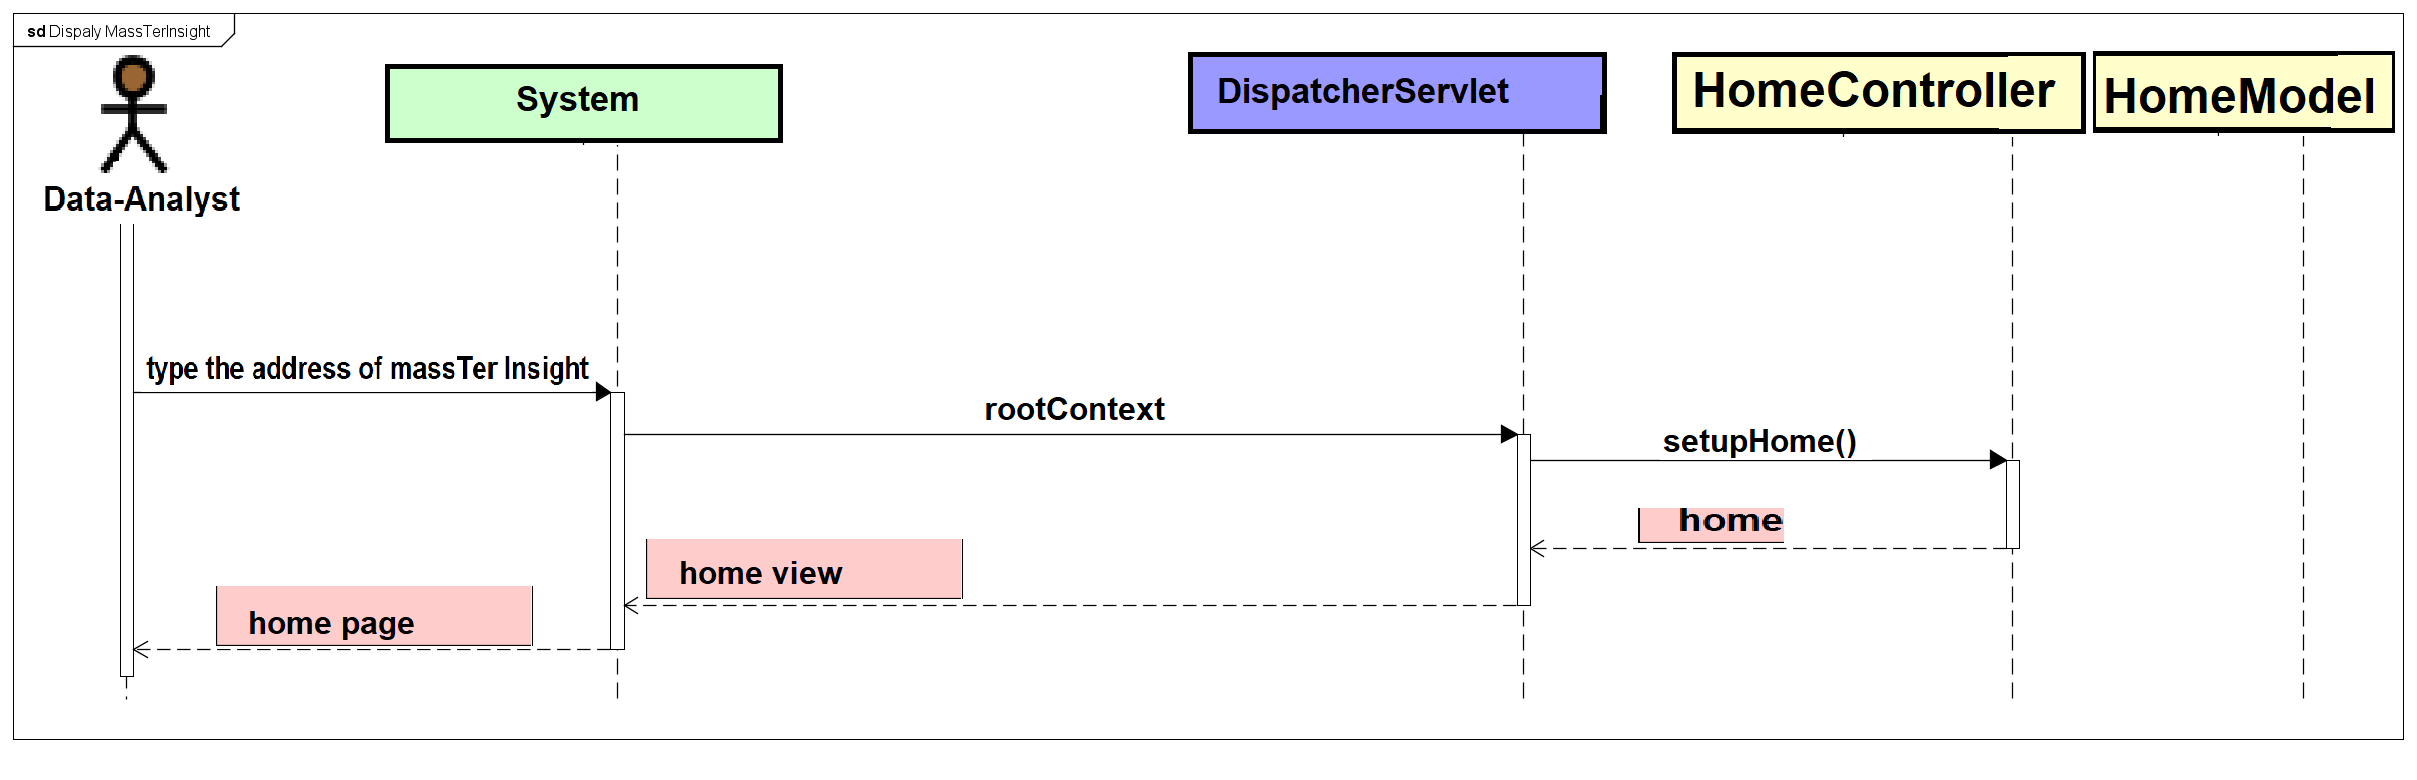
\includegraphics[width=17.5cm,height=8cm]{SequenceDiagramDispalyMassTerInsight.png}
		\caption{Sequence Diagram \textbf{Display MassTerInsight}}
		\end{figure}
	
	\pagebreak
	\clearpage
	\newpage
	\begin{figure}[h]
		\centering
		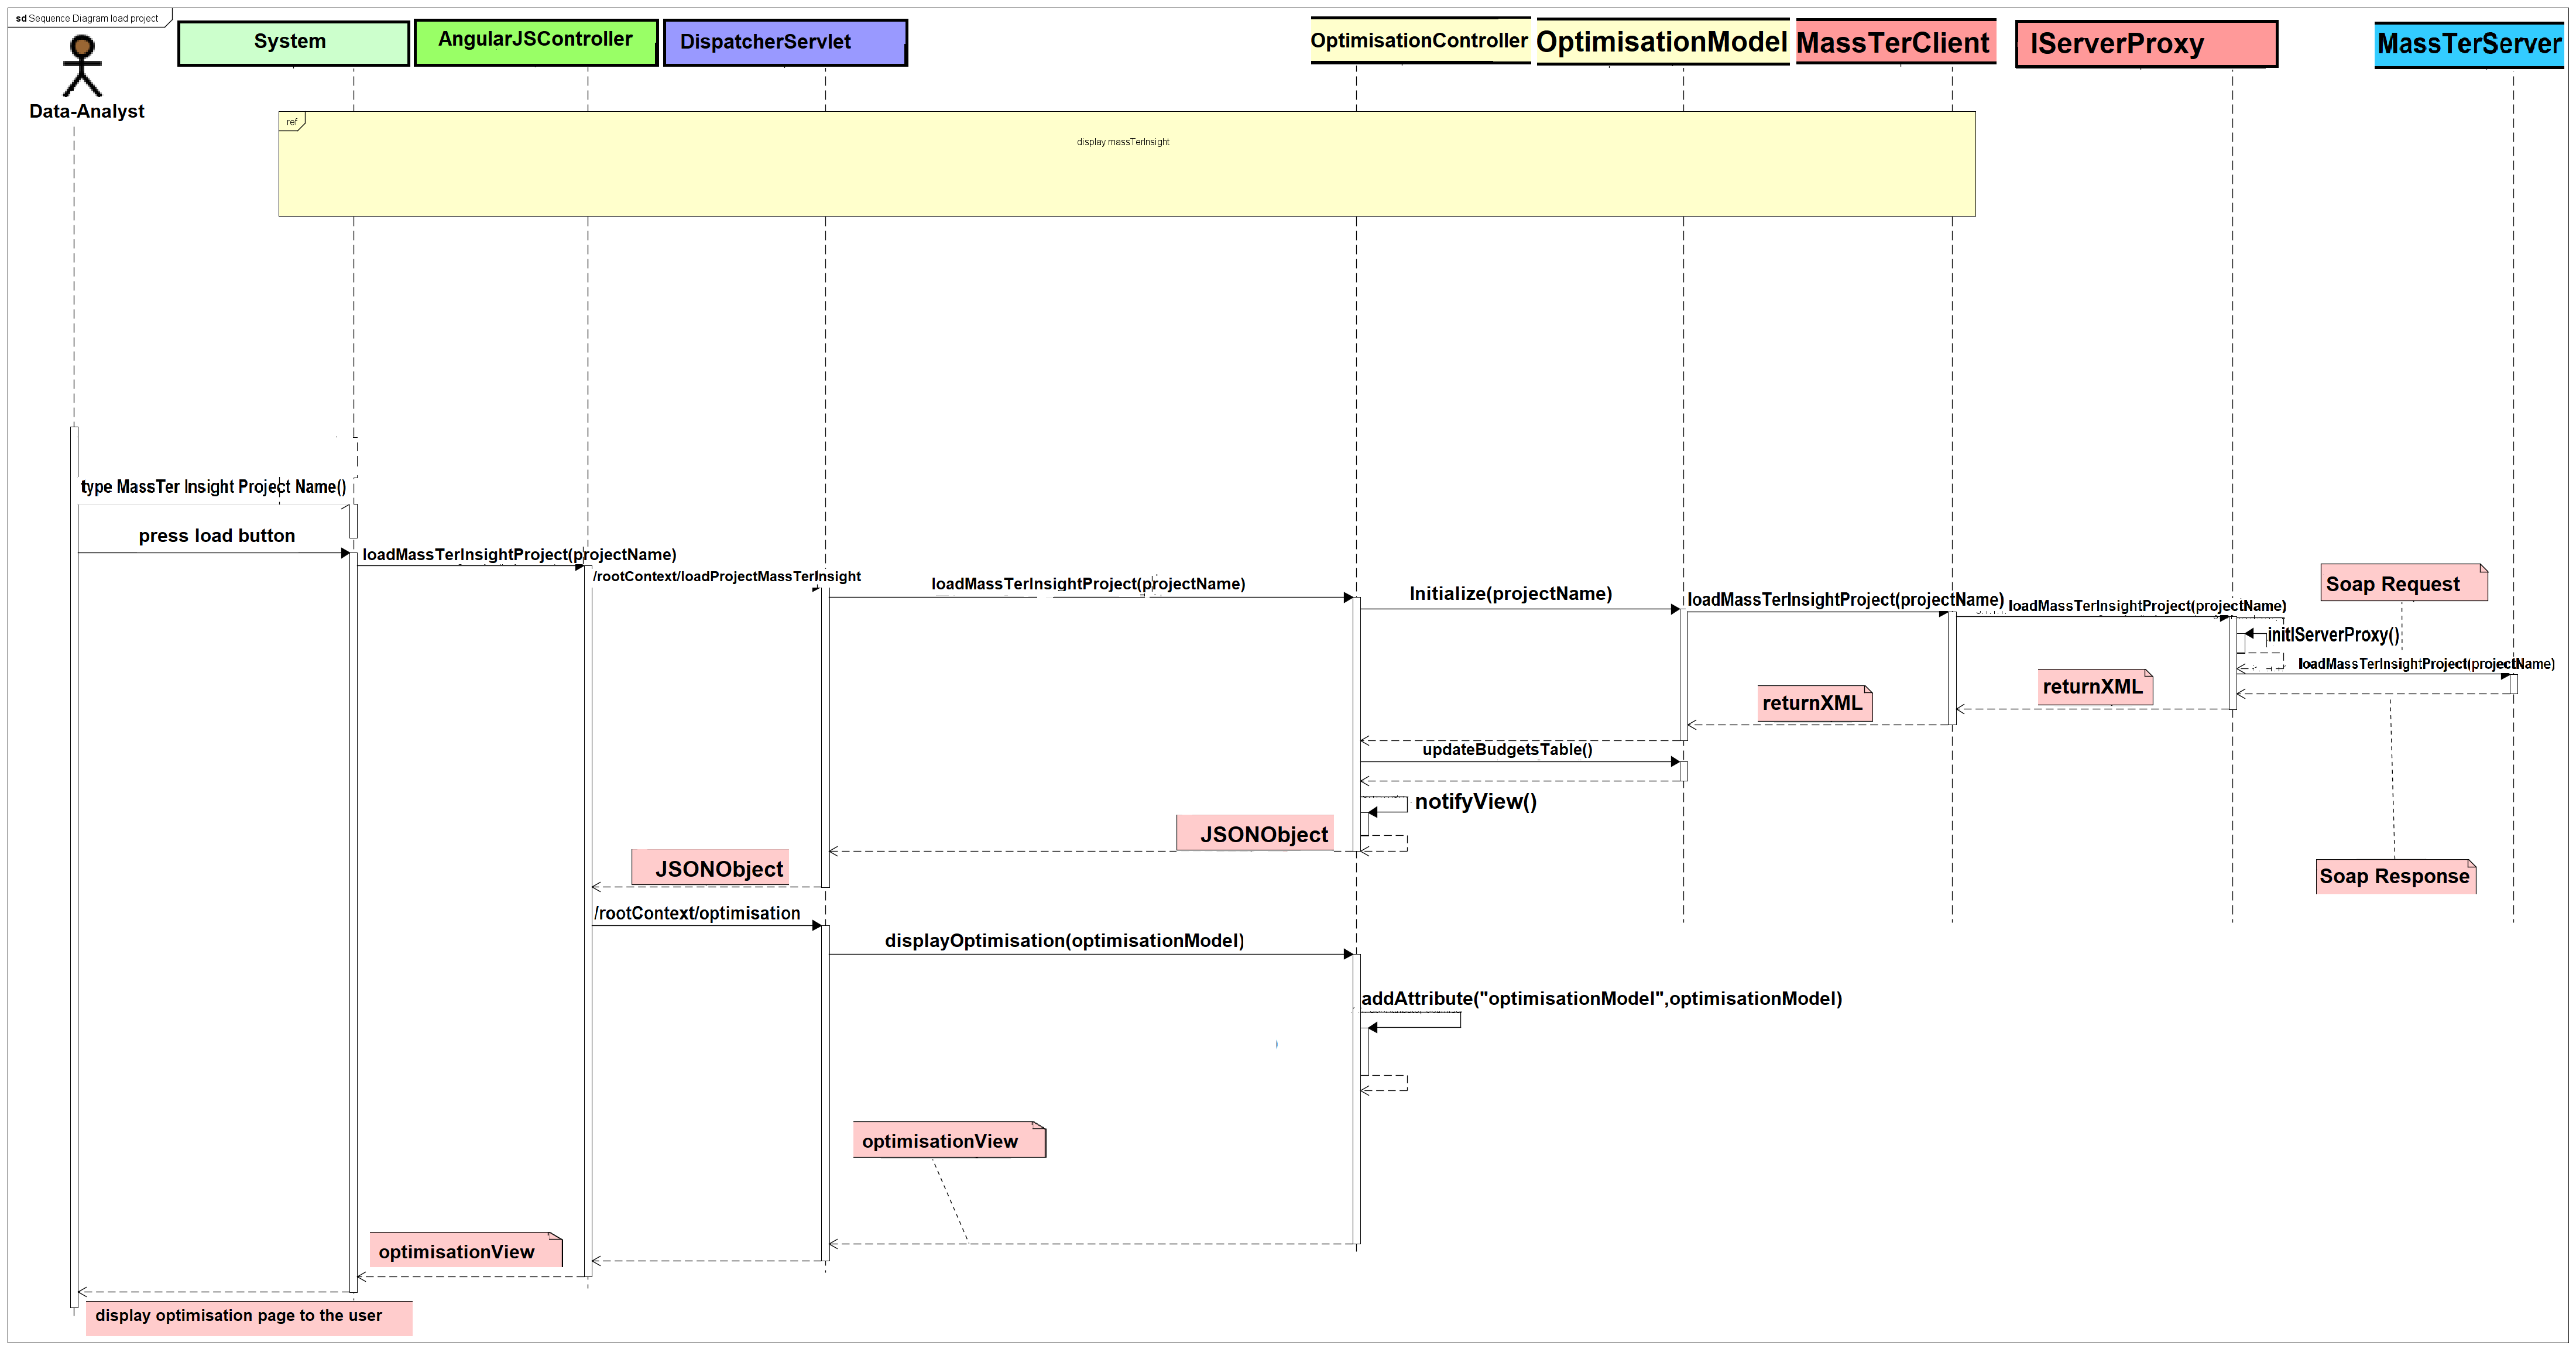
\includegraphics[width=17.5cm,height=17cm]{SequenceDiagramLoadProject.png}
		\caption{Sequence Diagram \textbf{Load MassTerInsight Project Use Case}}
	\end{figure}
    
    \pagebreak
	\clearpage
	\newpage

	\begin{figure}[h]
		\centering
		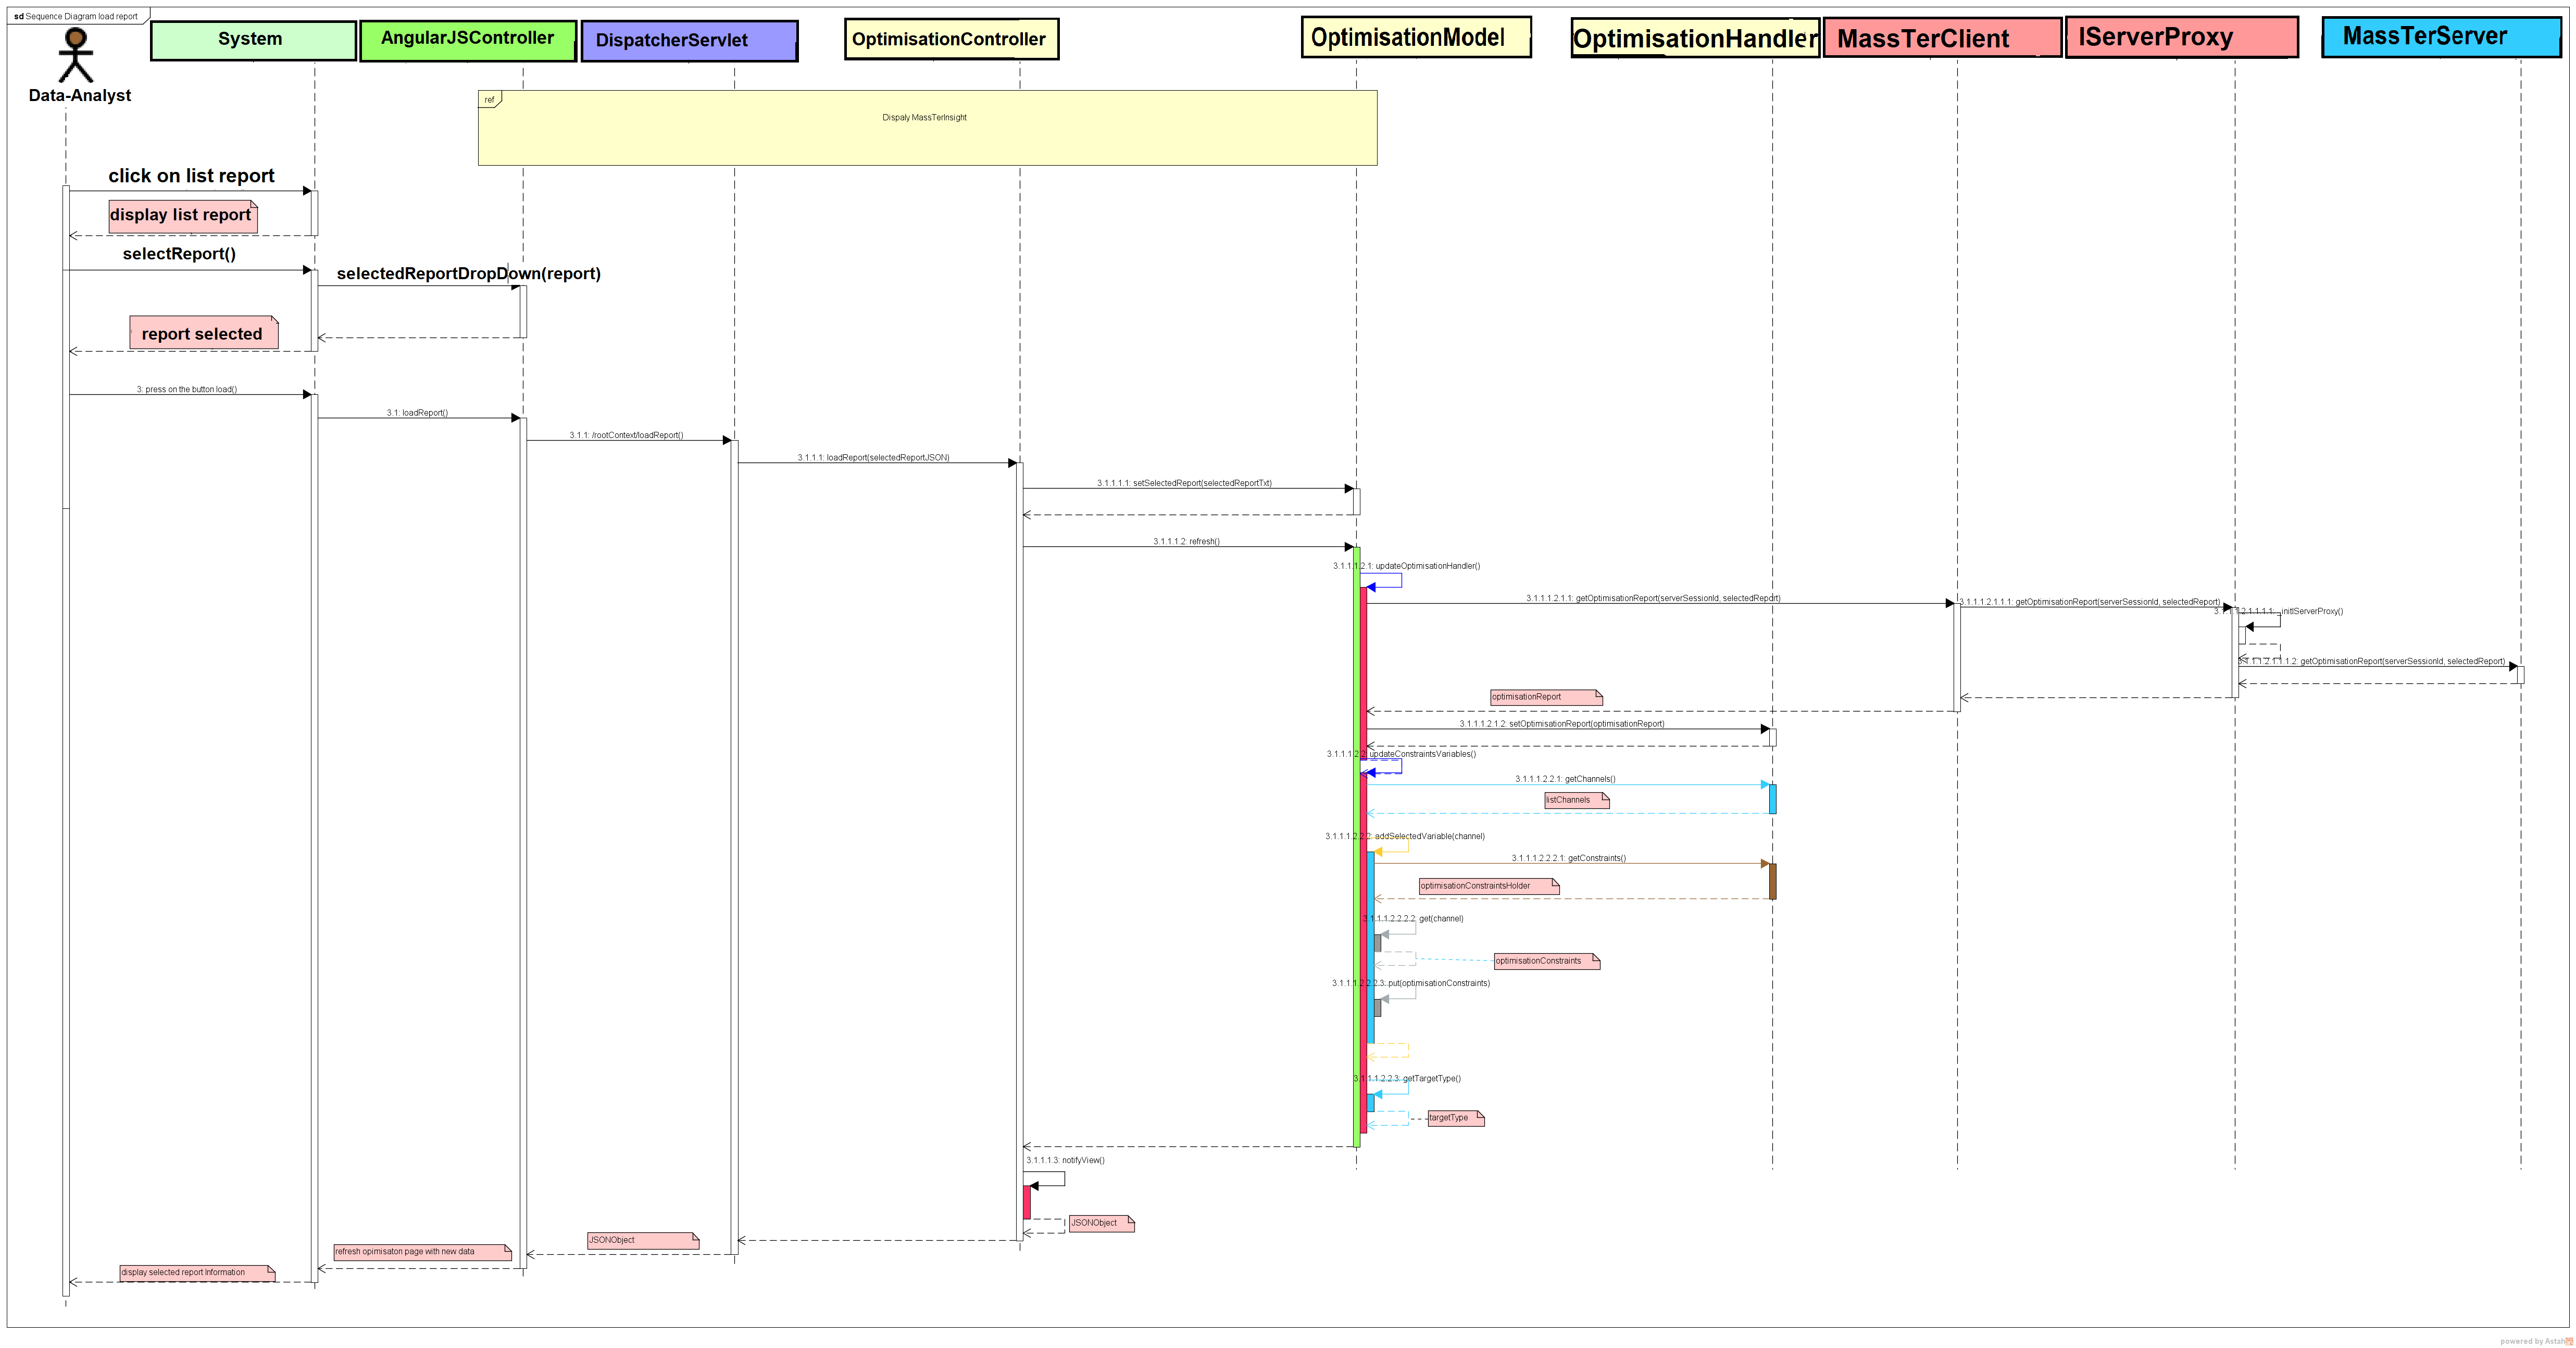
\includegraphics[width=17.5cm,height=17cm]{SequenceDiagramLoadReport.png}
		\caption{Sequence Diagram \textbf{Load Report Use Case}}
	\end{figure}


	\pagebreak
	\clearpage
	\newpage

	\begin{figure}[h]
		\centering
		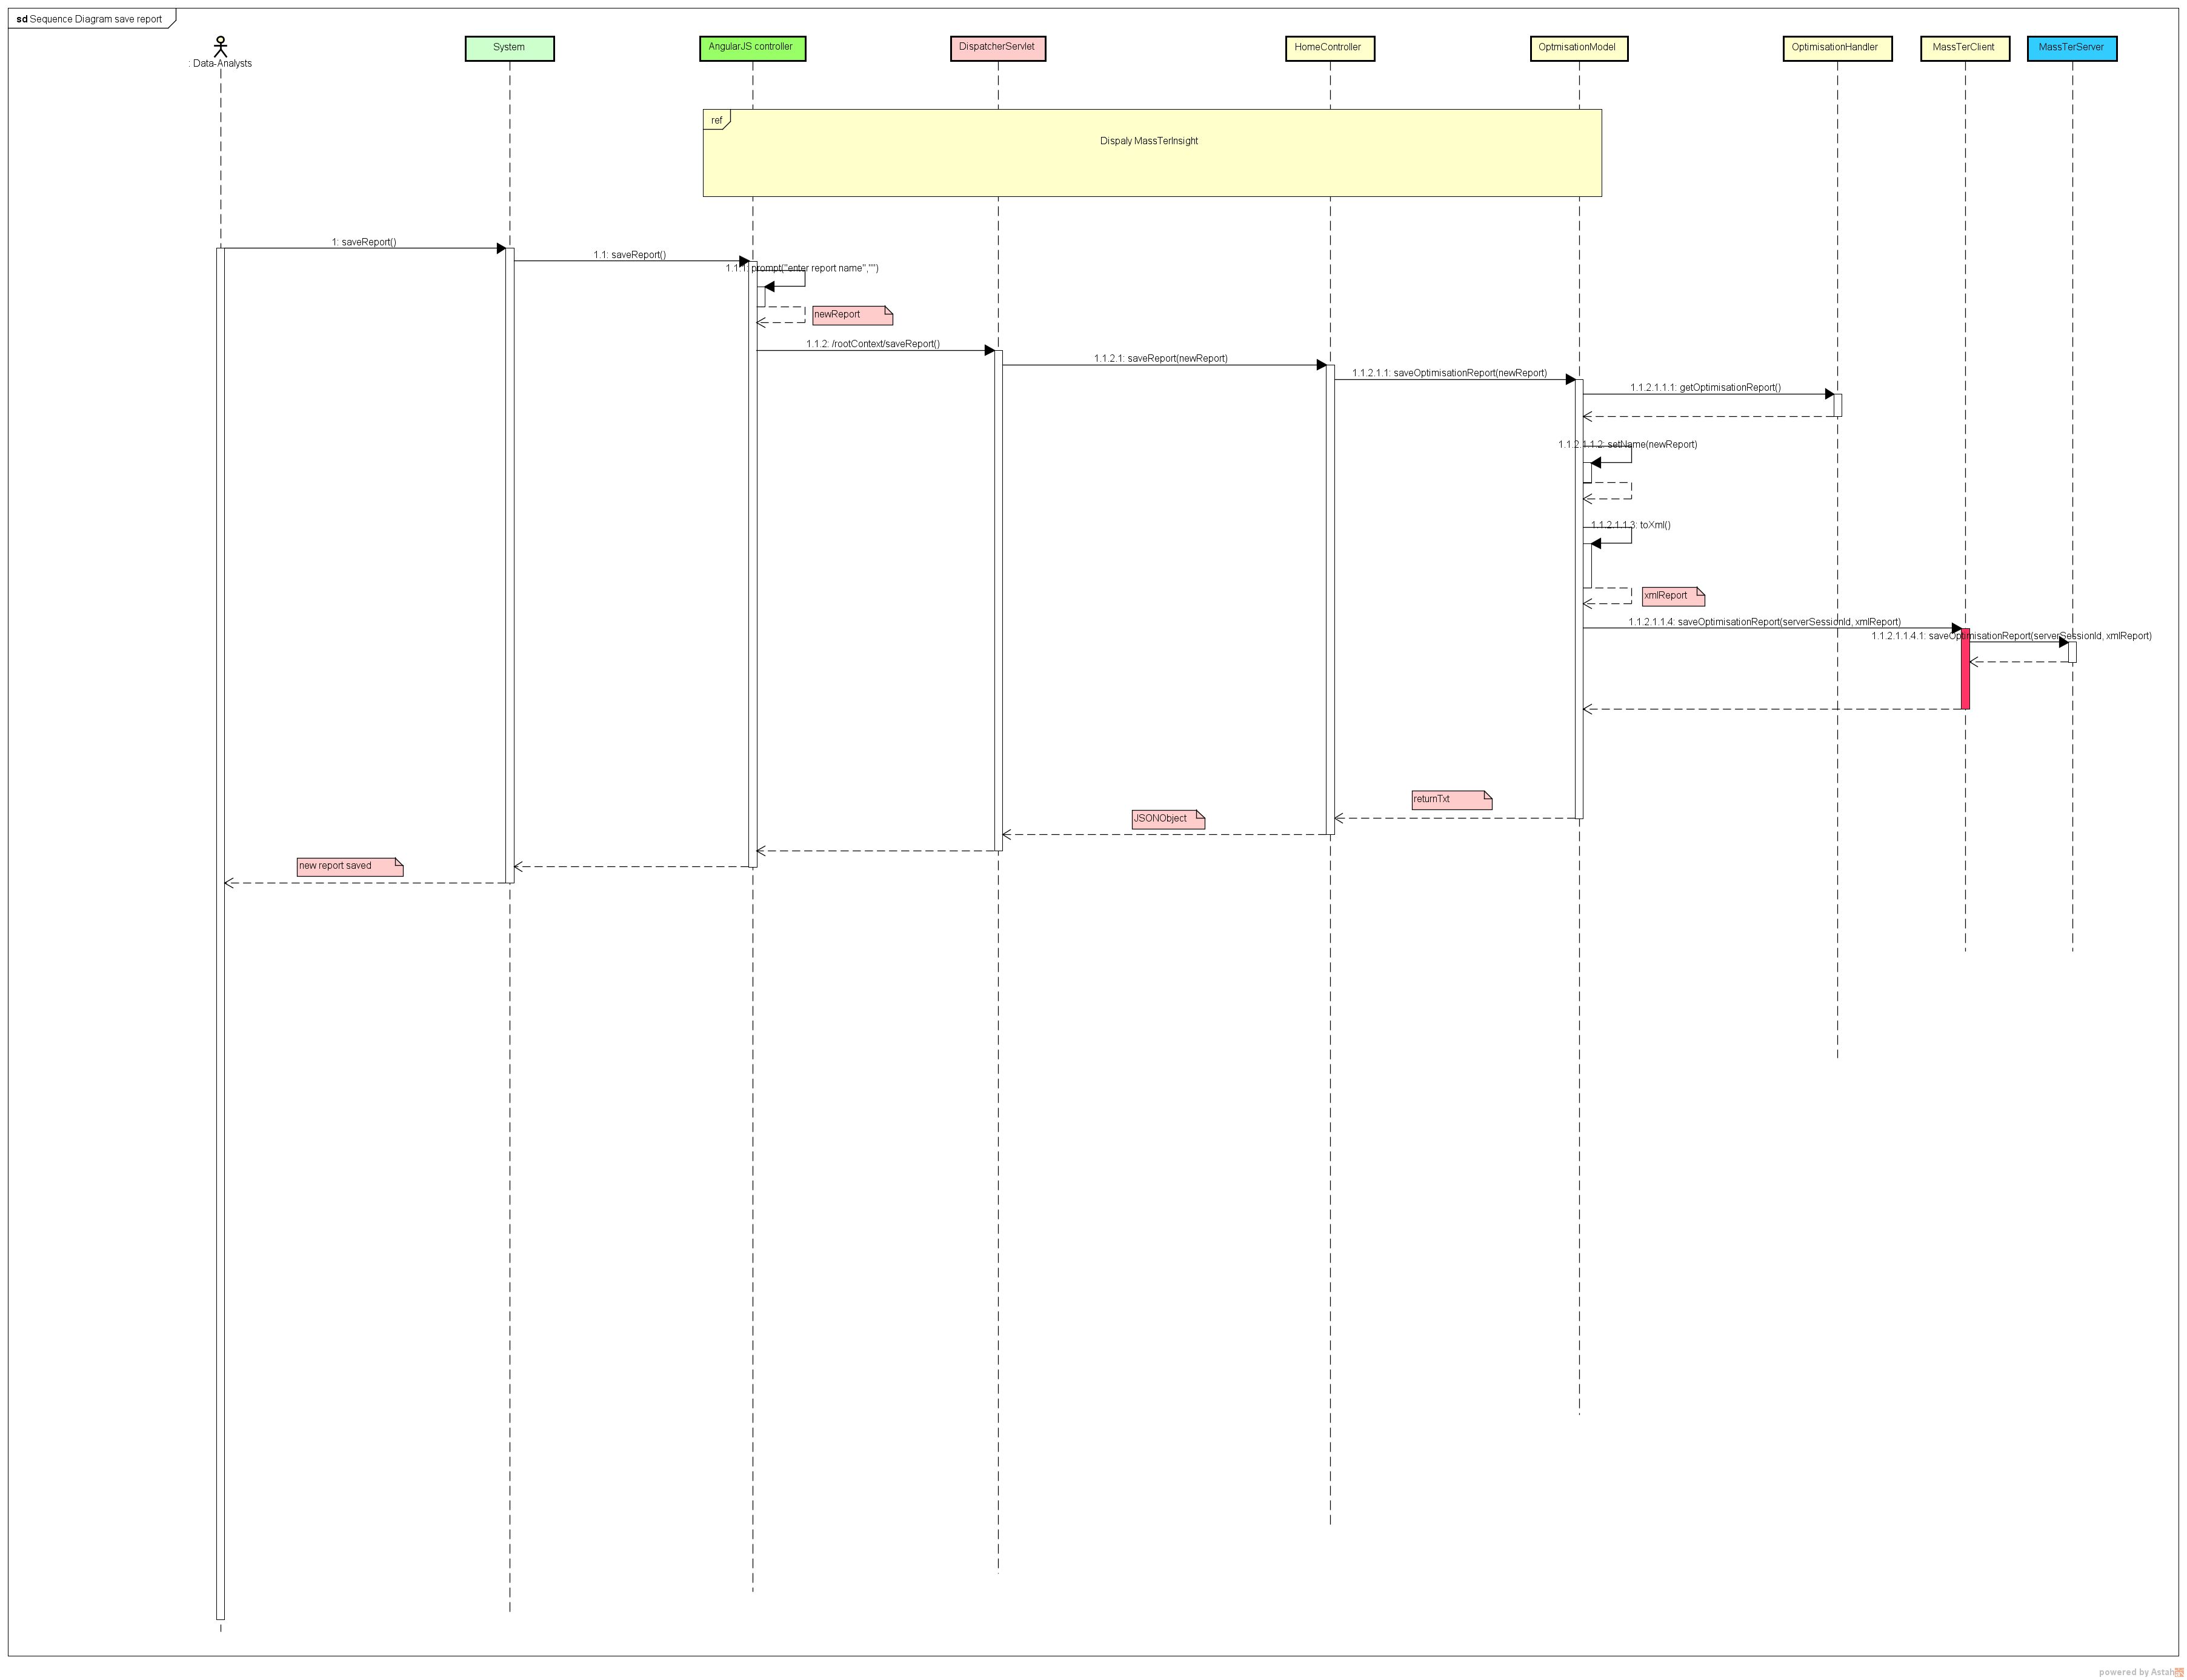
\includegraphics[width=17.5cm,height=17cm]{SequenceDiagramSaveReport.png}
		\caption{Sequence Diagram \textbf{Save Report Use Case}}
	\end{figure}
	
	\pagebreak
	\clearpage
	\newpage 

   \begin{figure}[h]
   	\centering
   	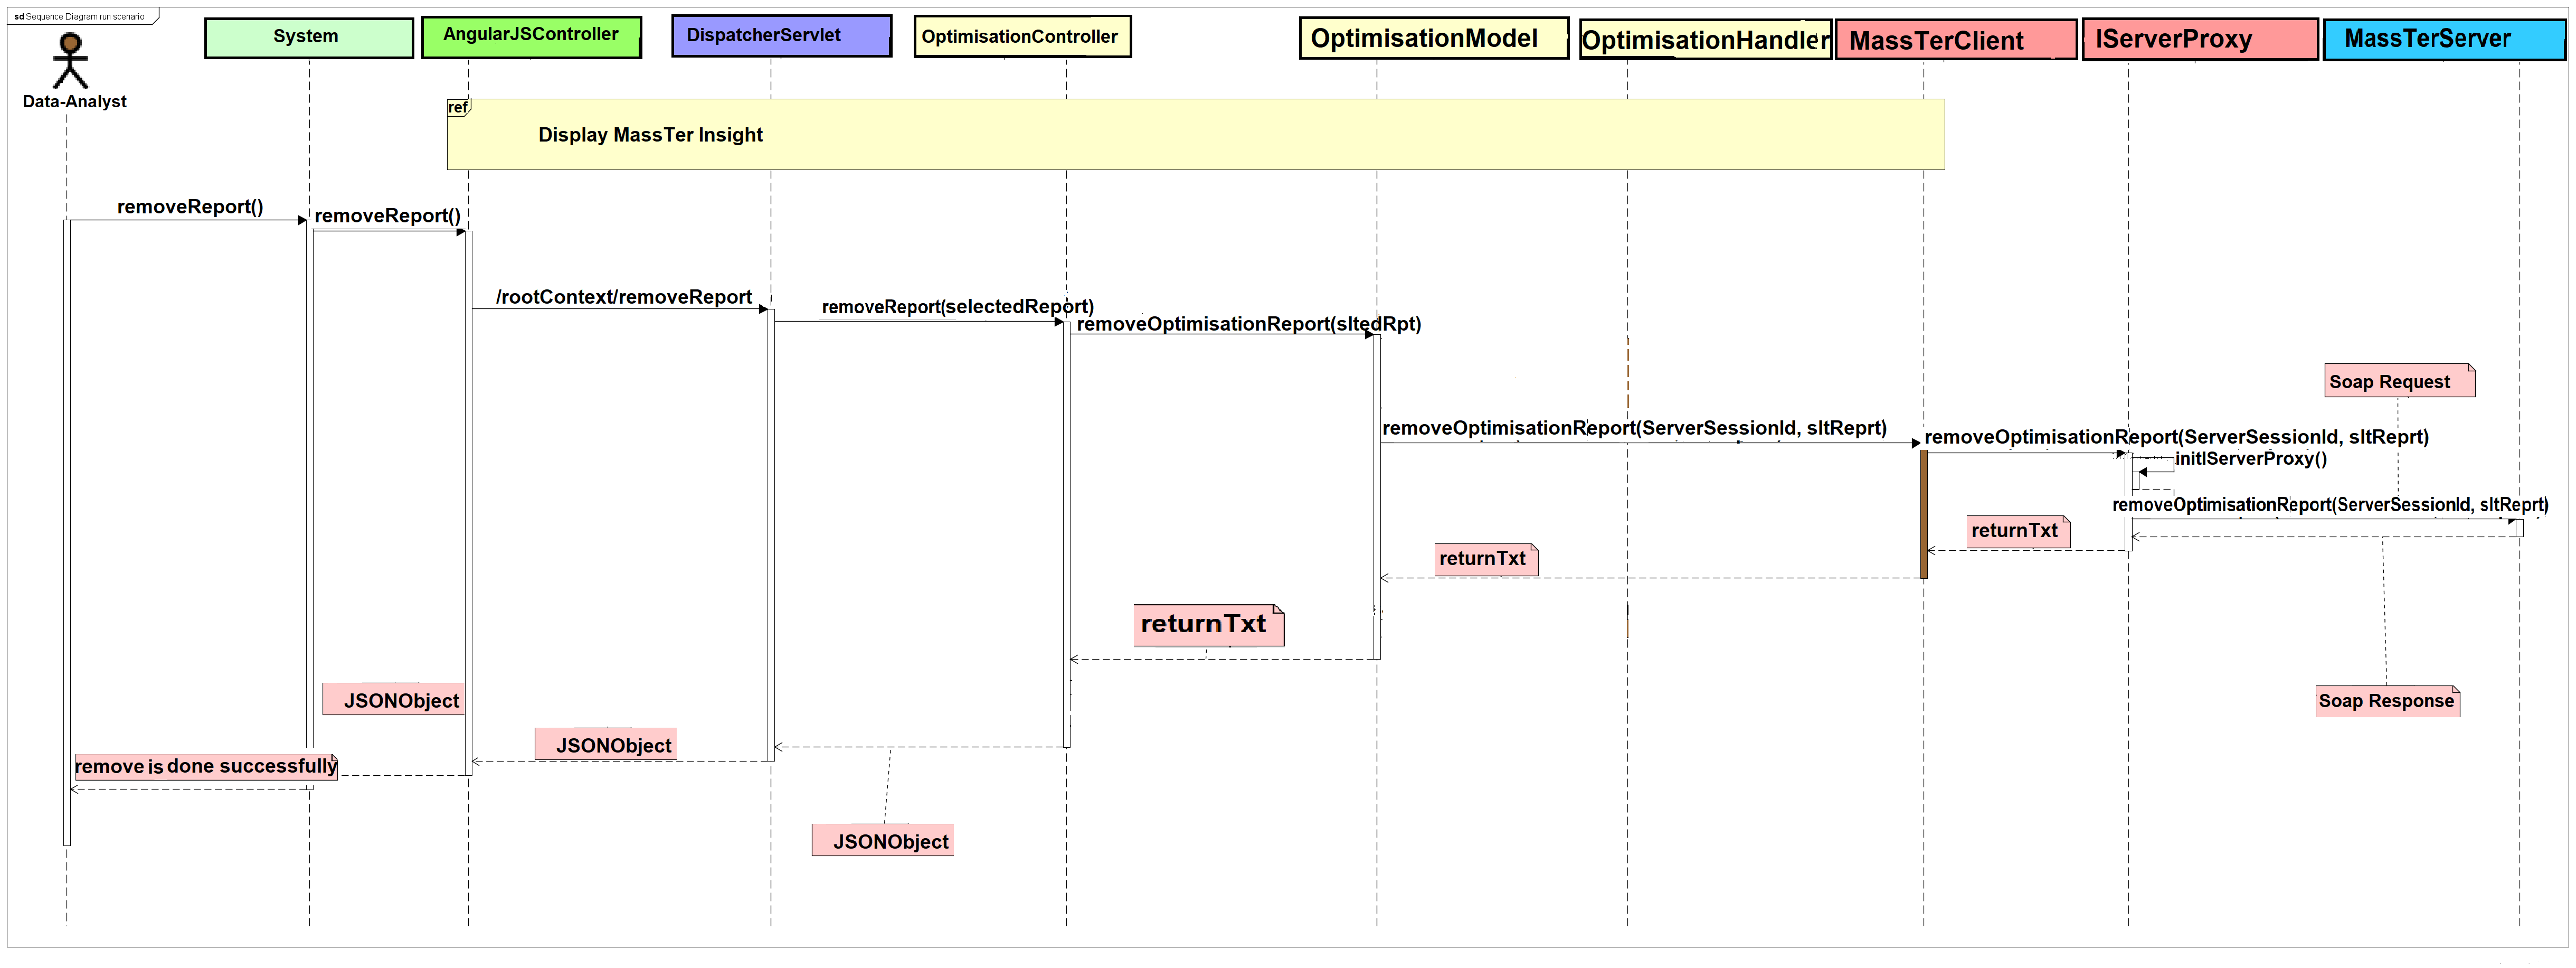
\includegraphics[width=17.5cm,height=17cm]{SequenceDiagramRemoveReport.png}
   	\caption{Sequence Diagram \textbf{Remove Report Use Case}}
   \end{figure}
	
	\pagebreak
	\clearpage
	\newpage
	
	\begin{figure}[h]
		\centering
		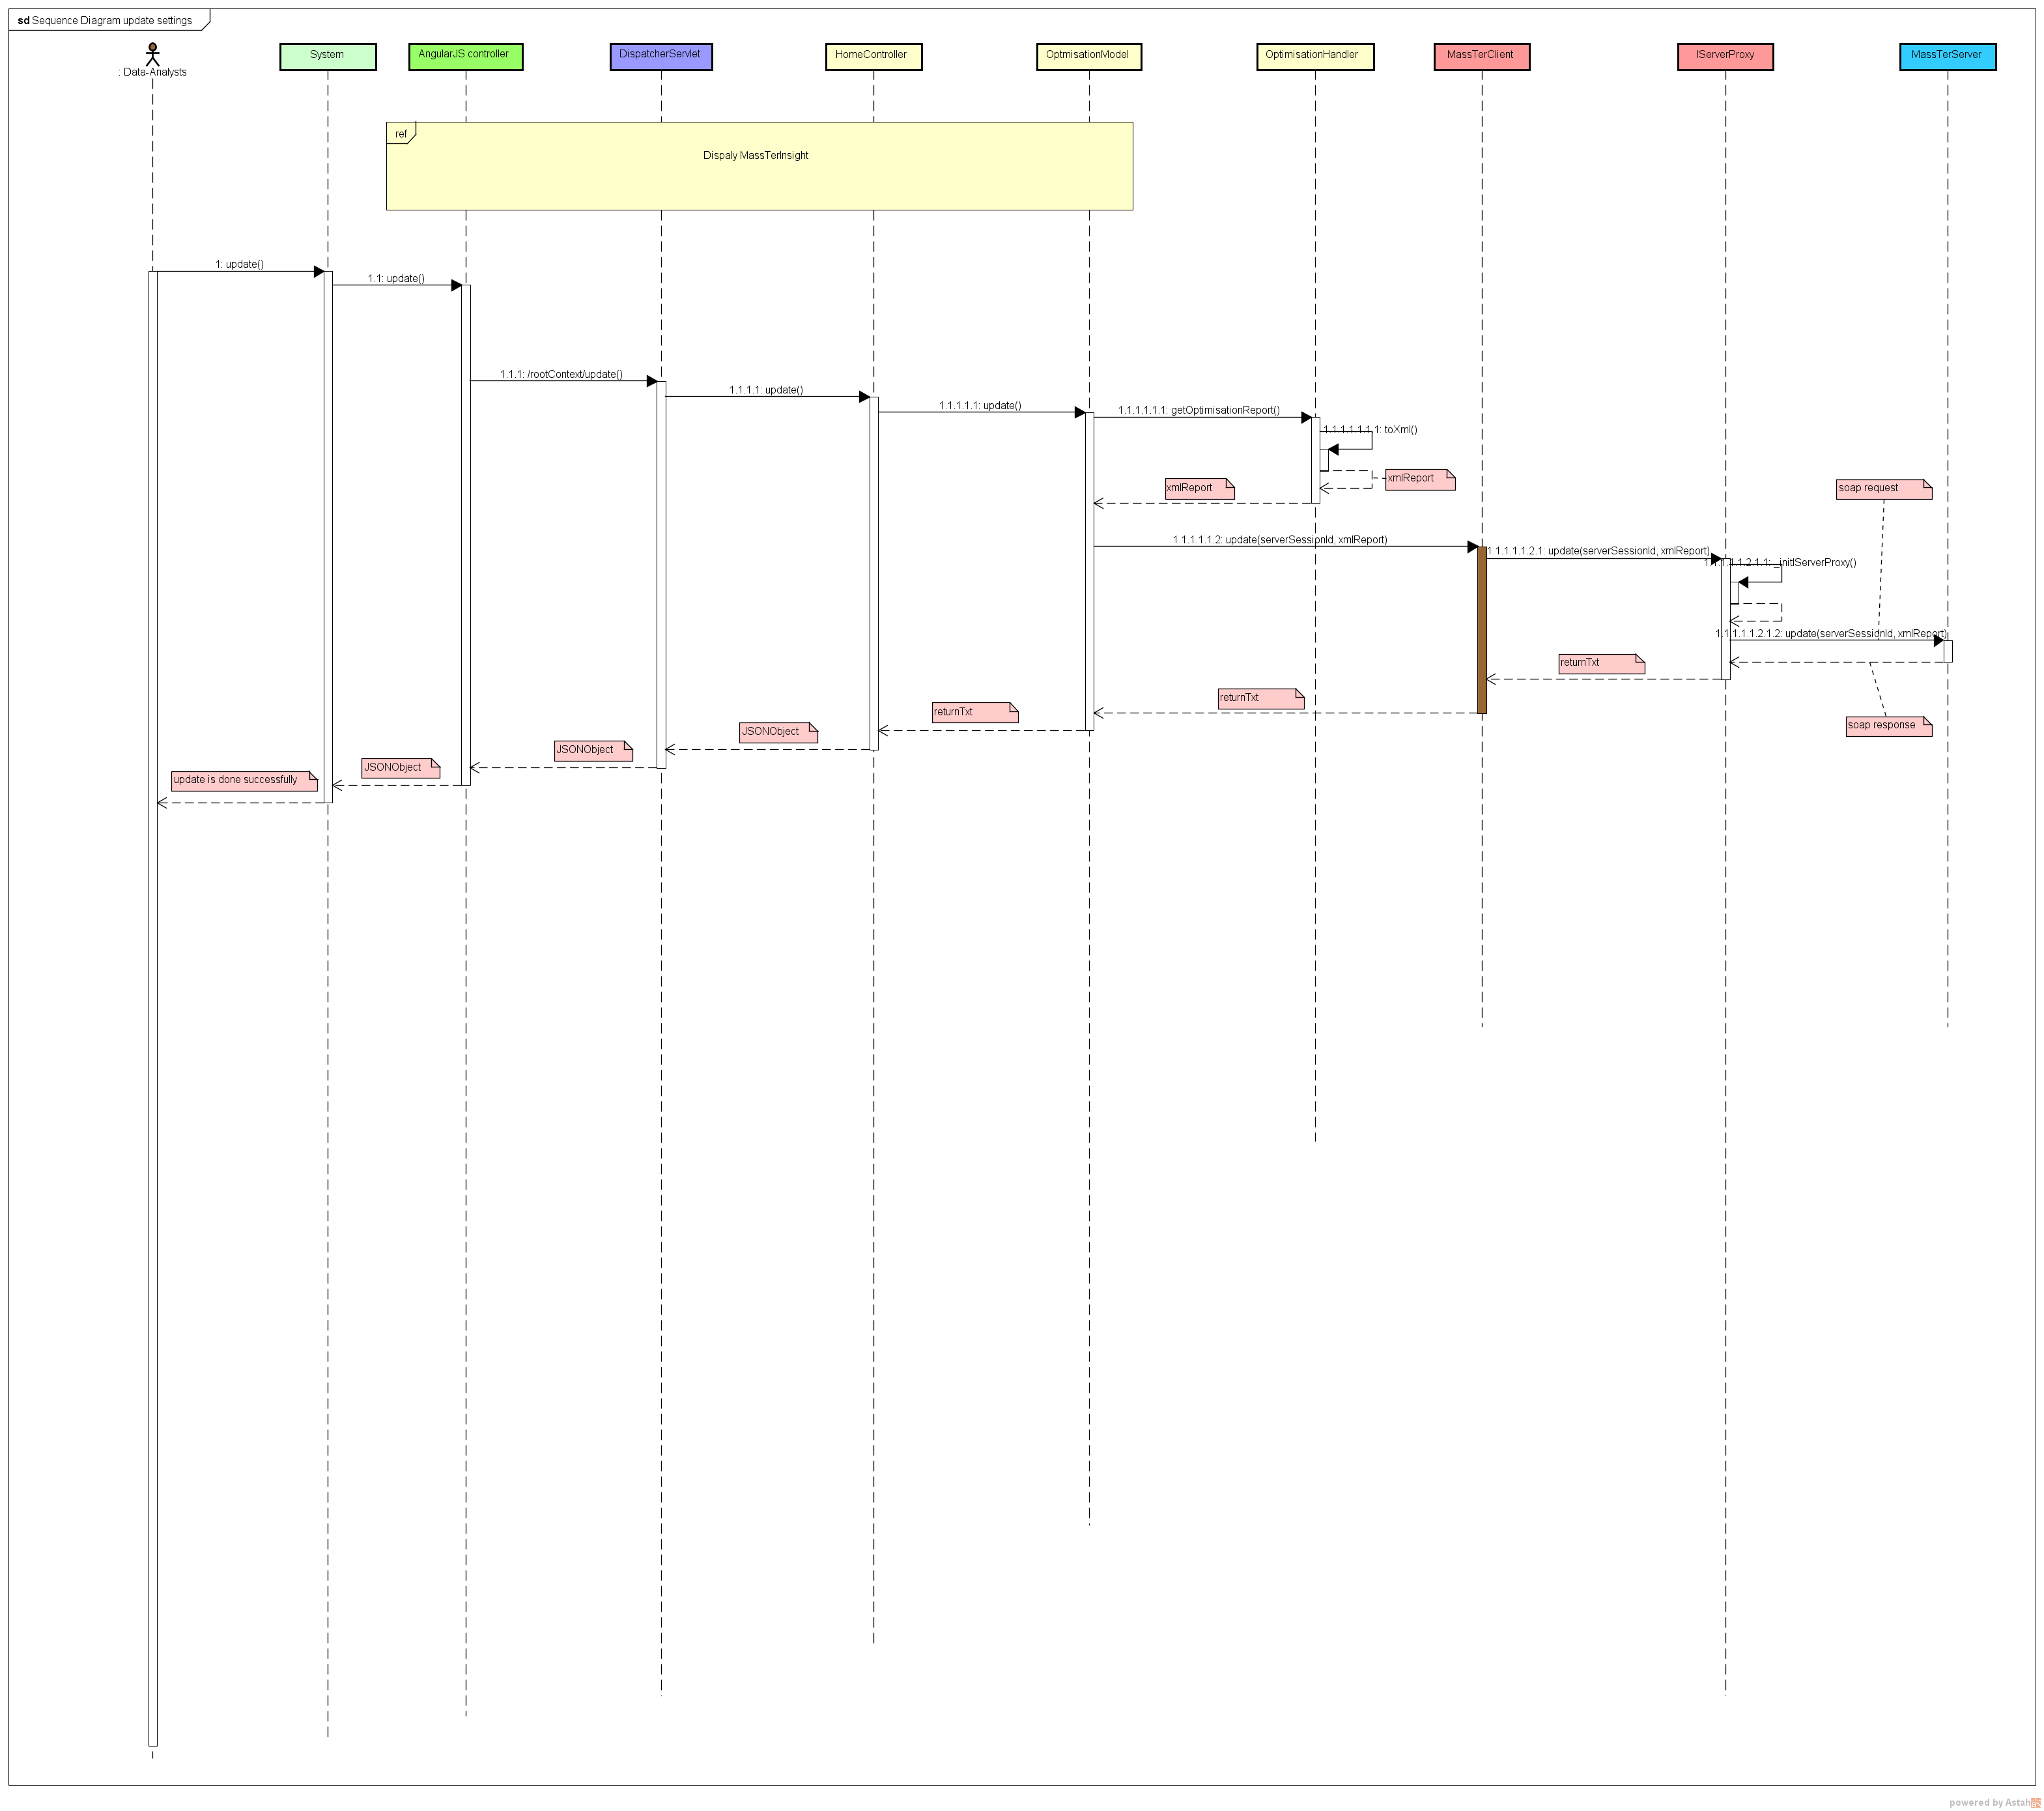
\includegraphics[width=17.5cm,height=17cm]{SequenceDiagramUpdateSettings.png}
		\caption{Sequence Diagram \textbf{update settings Use Case}}
	\end{figure}

	
	\pagebreak
	\clearpage
	\newpage
	
	\begin{figure}[h]
	\centering
	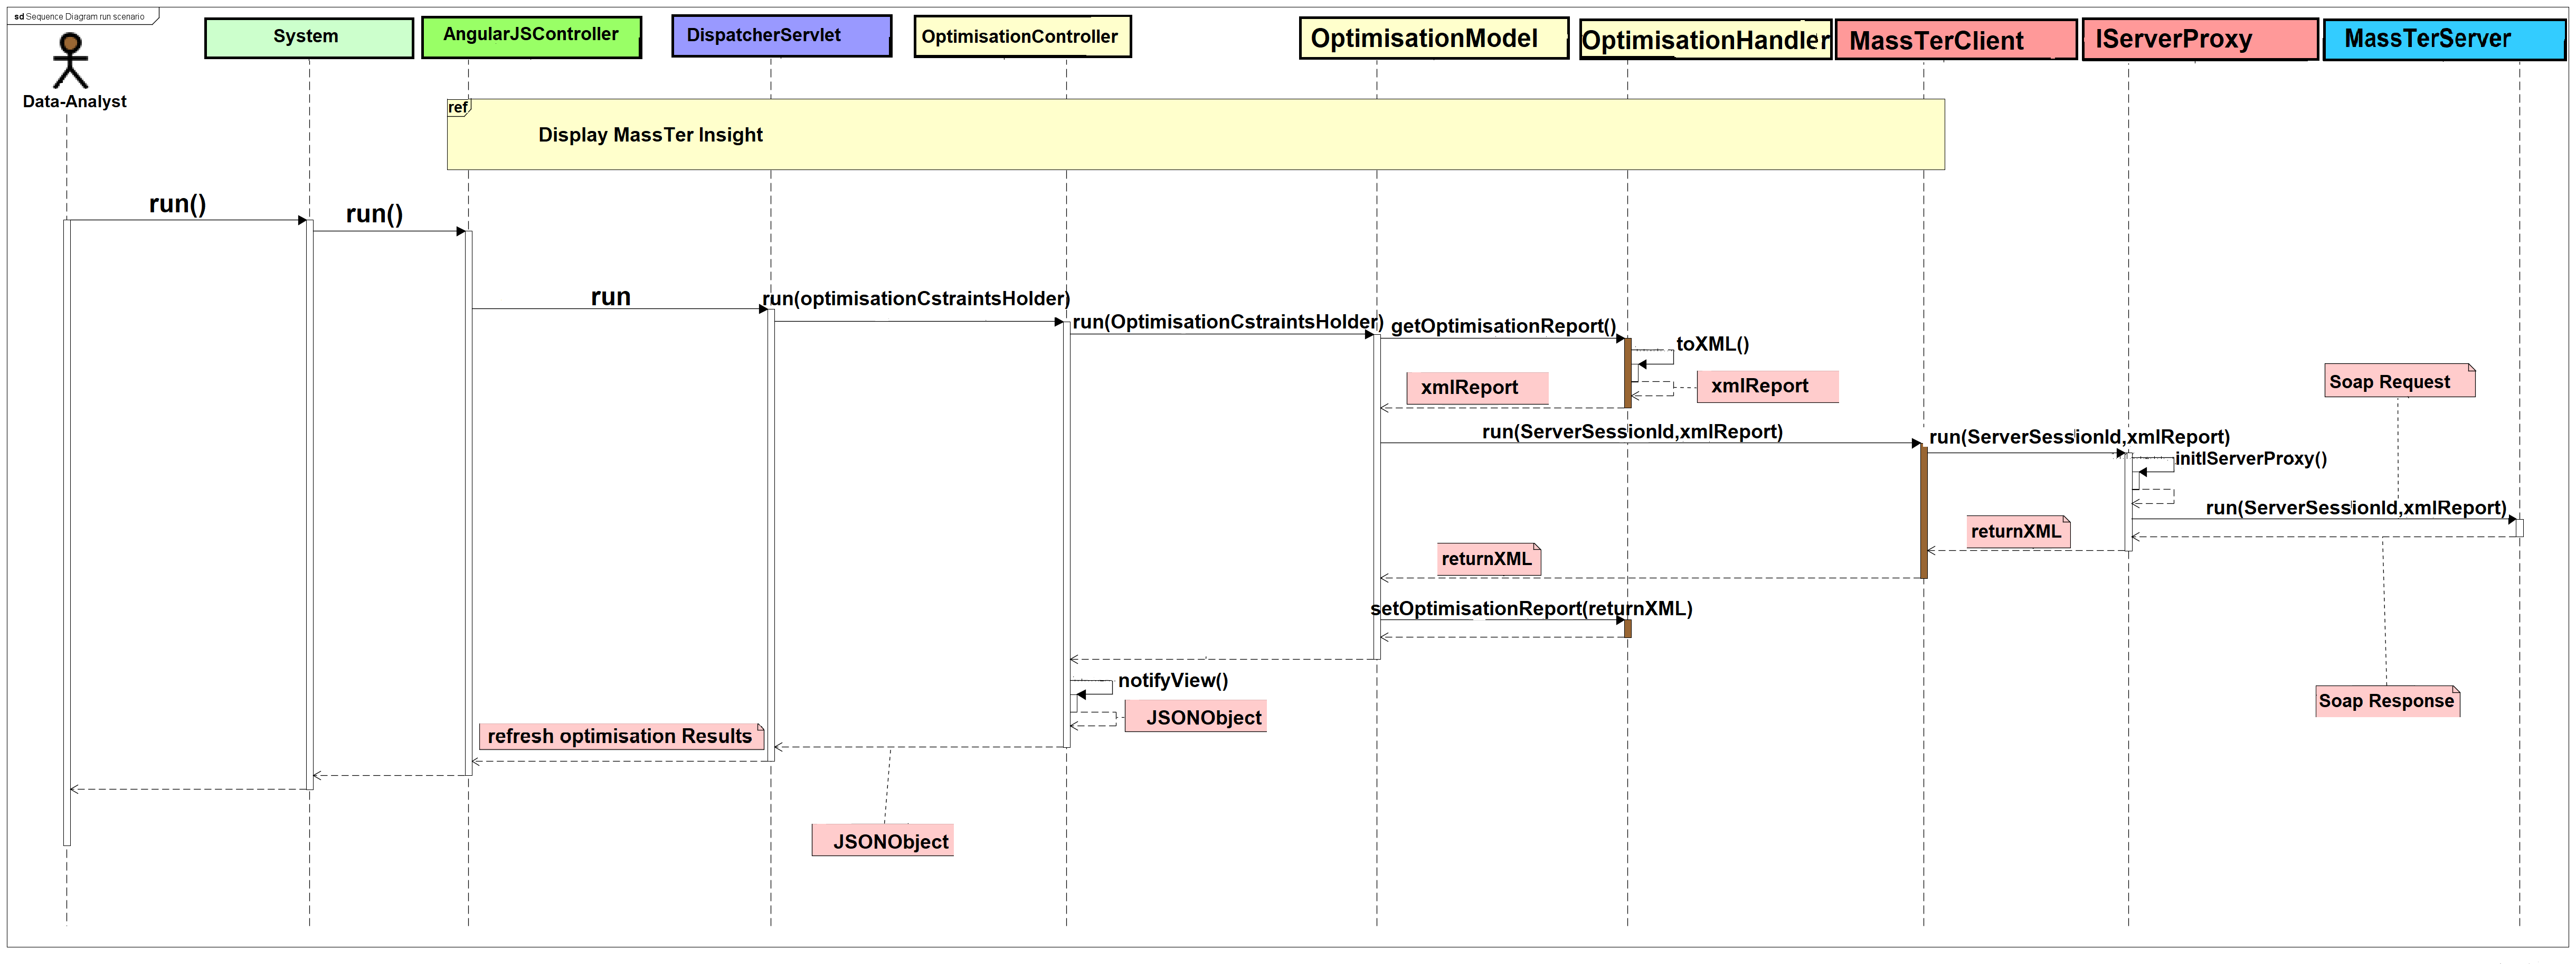
\includegraphics[width=17.5cm,height=17cm]{SequenceDiagramRunScenario.png}
	\caption{Sequence Diagram \textbf{Run Scenario Use Case}}
    \end{figure}
	
	\pagebreak
	\clearpage
    \newpage 
	
	\begin{figure}[h]
		\centering
		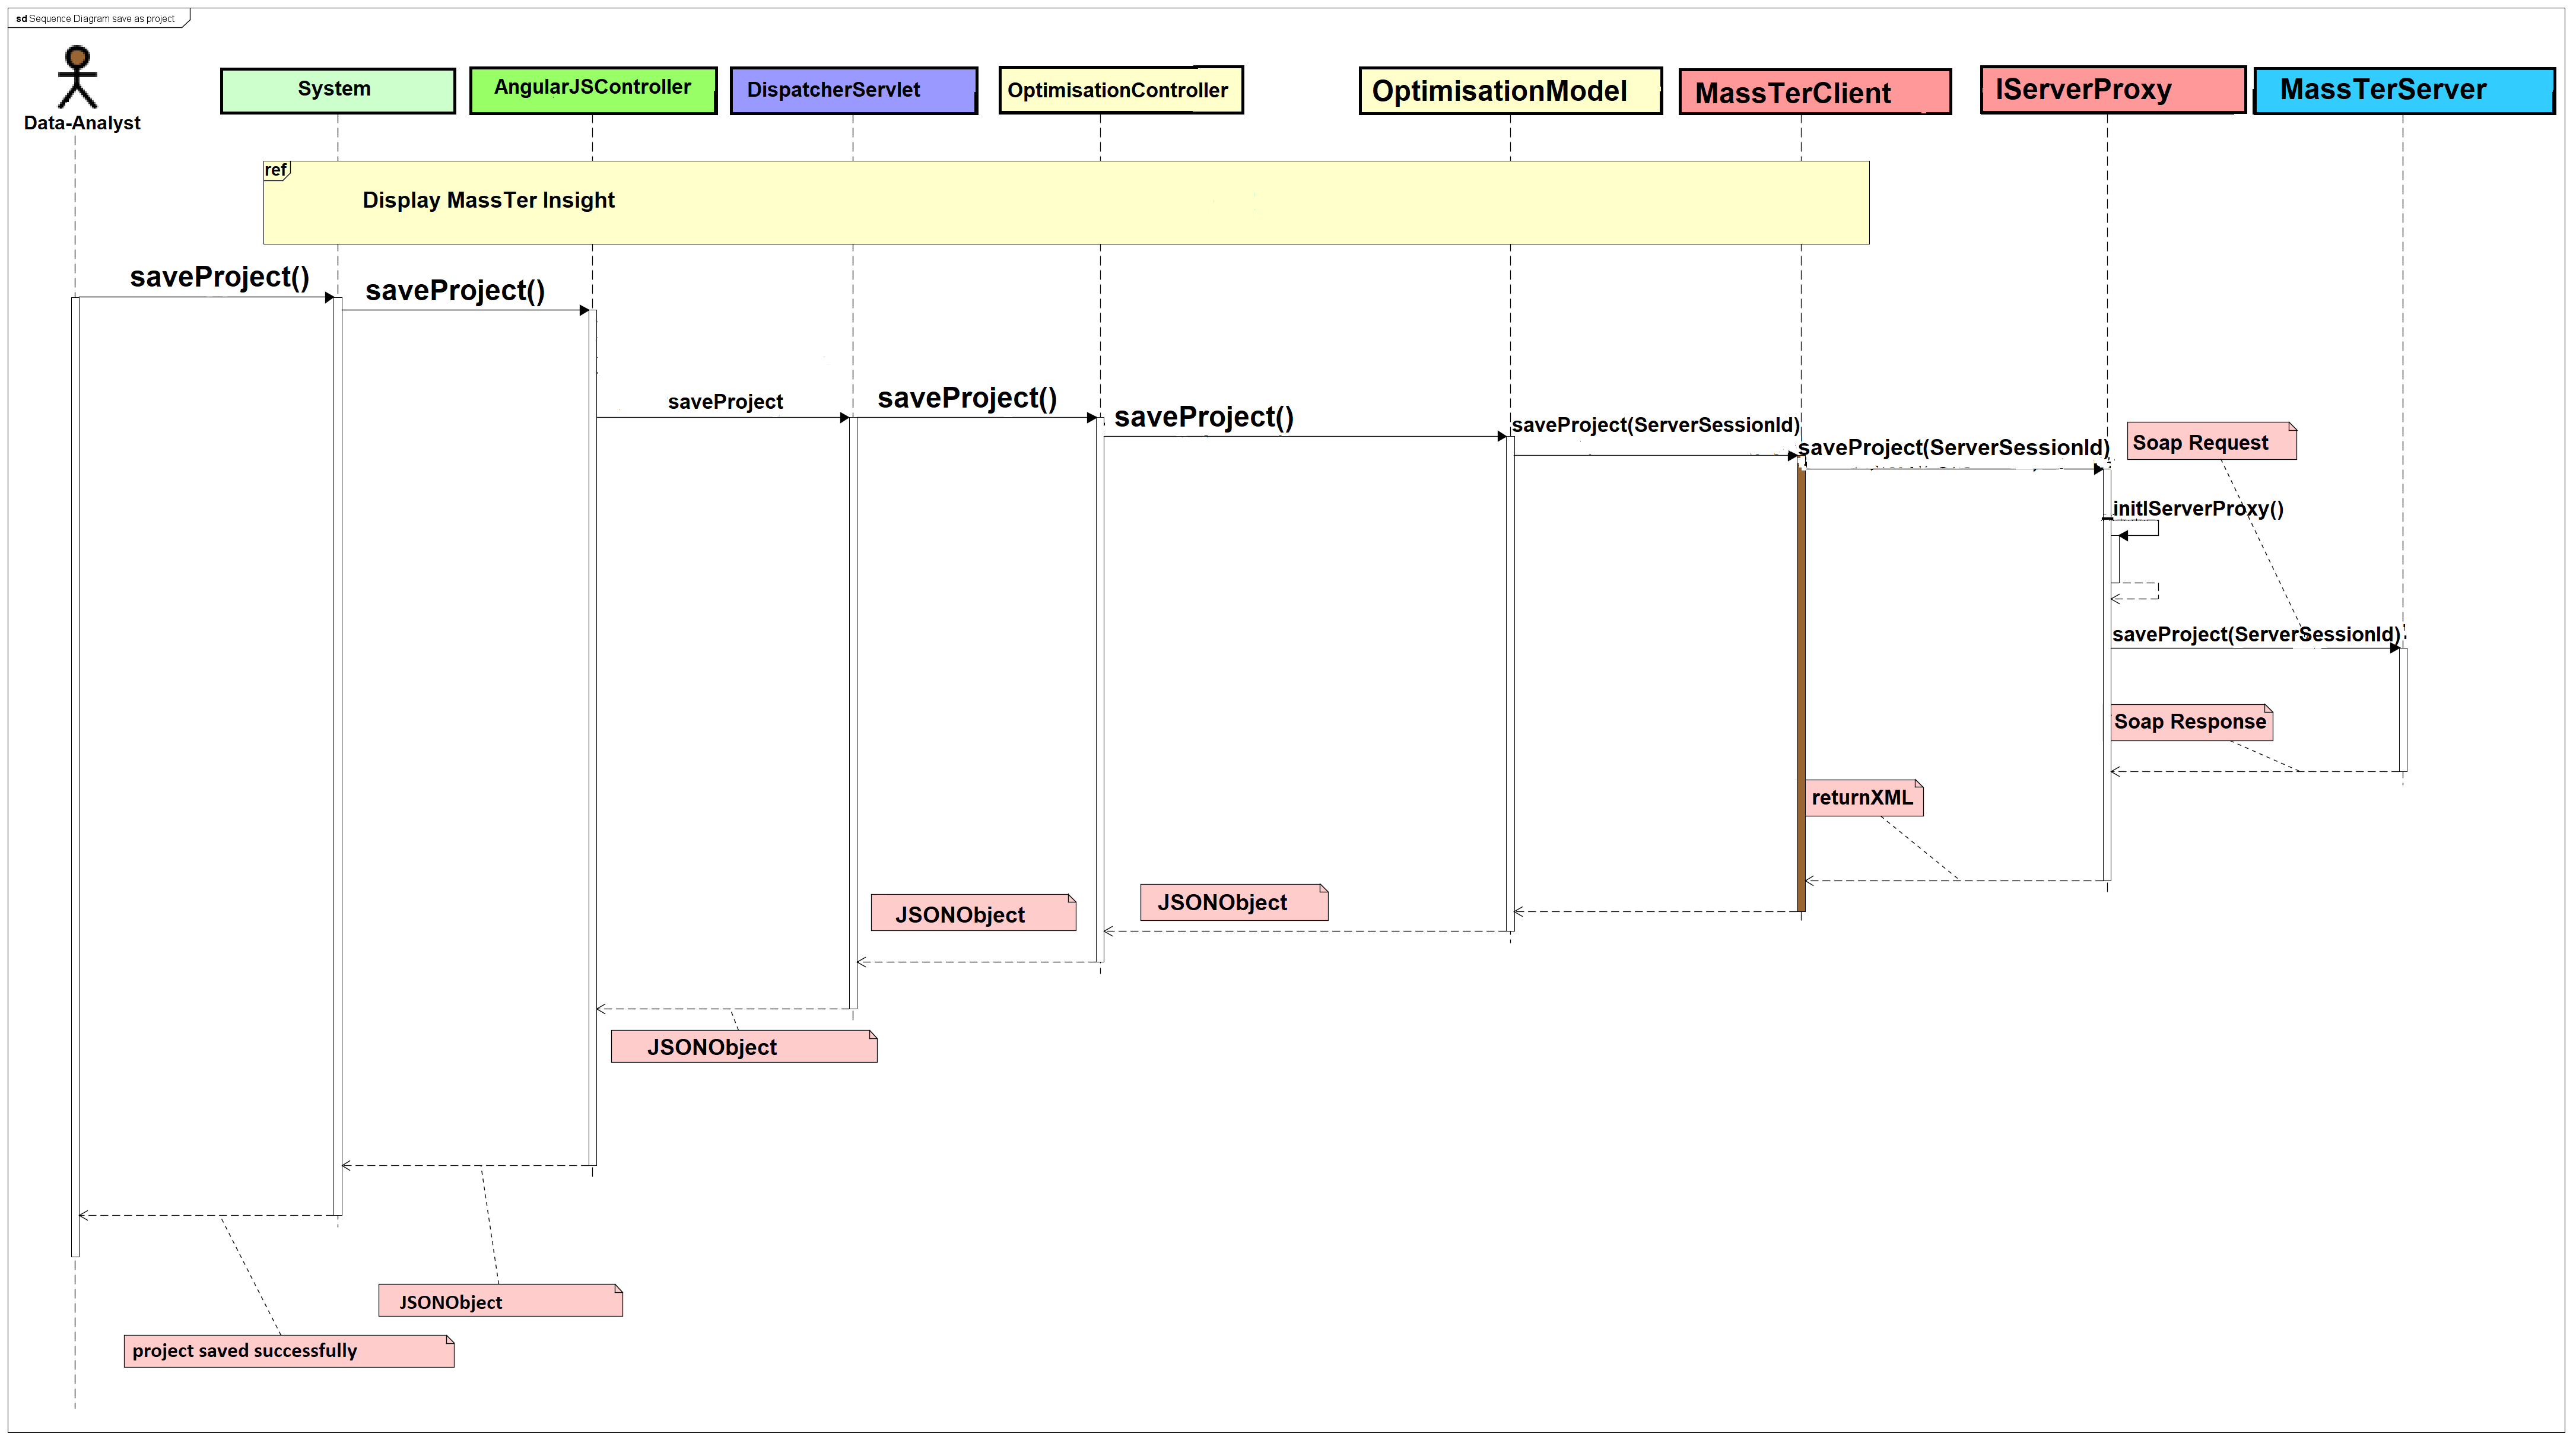
\includegraphics[width=17.5cm,height=17cm]{SequenceDiagramSaveProject.png}
		\caption{Sequence Diagram \textbf{Save Project Use Case}}
	\end{figure}

	
    \pagebreak
	\clearpage
	\newpage
	\begin{figure}[h]
	\centering
	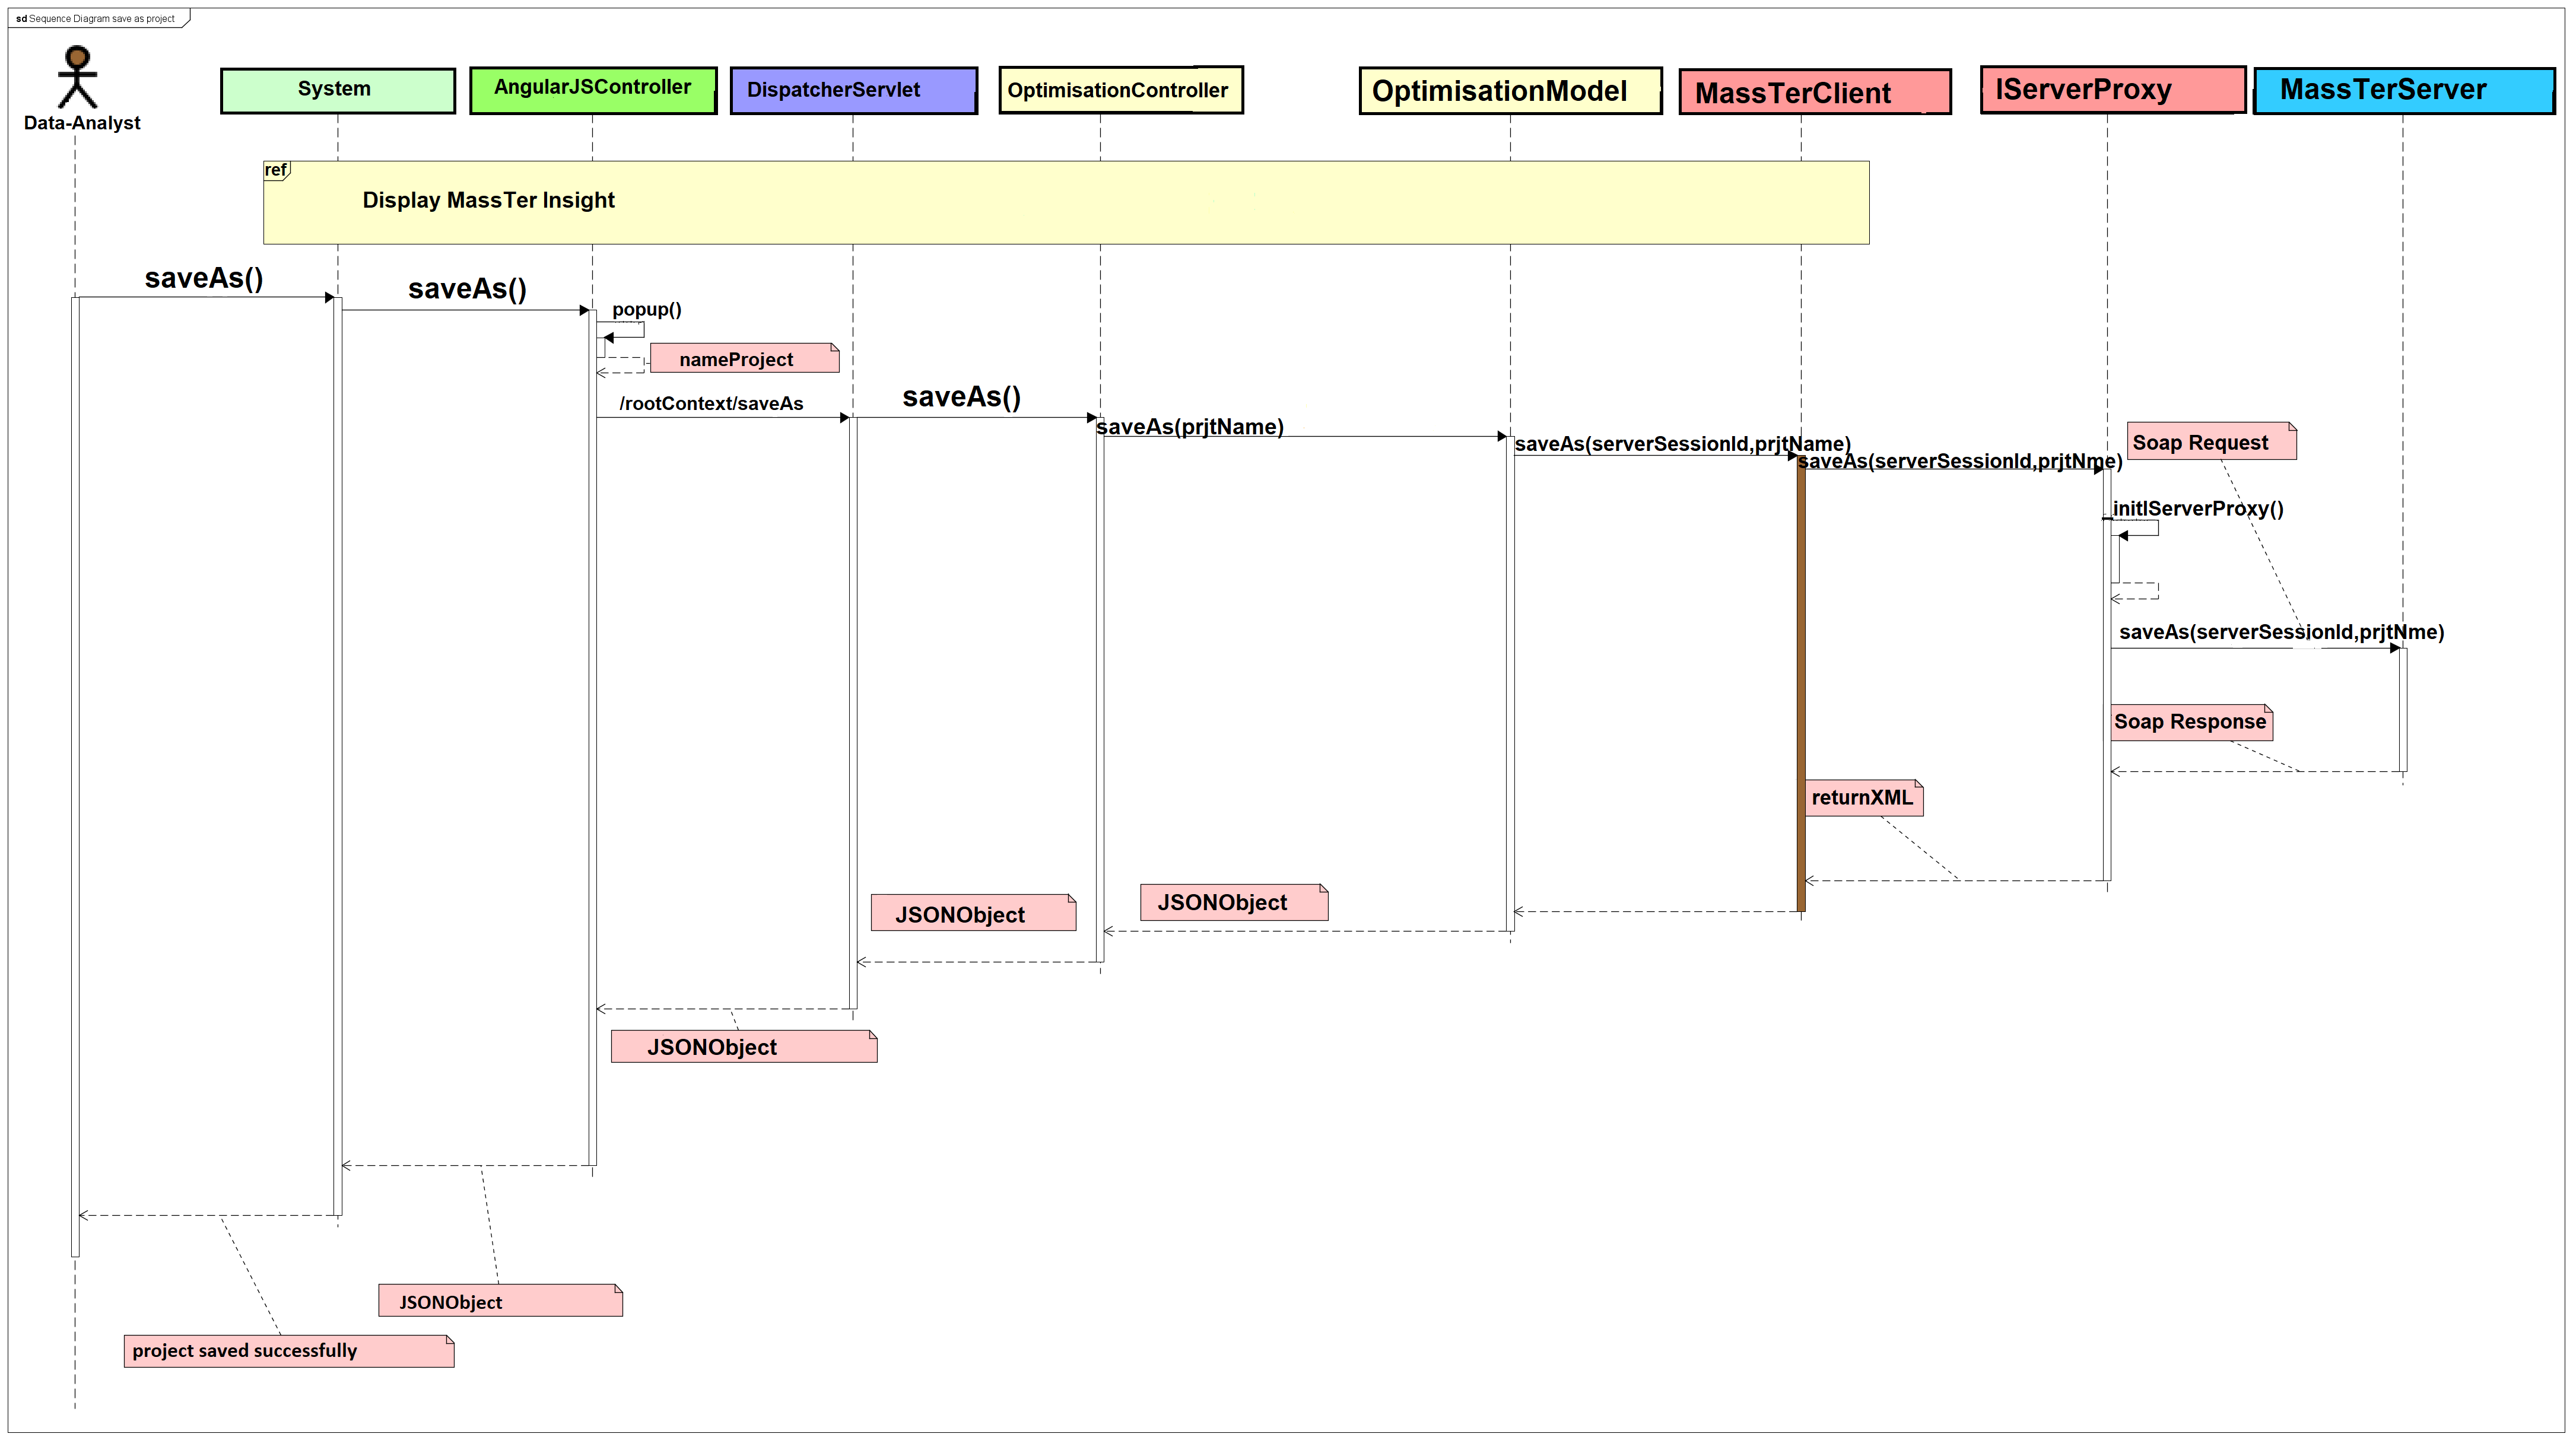
\includegraphics[width=17.5cm,height=17cm]{SequenceDiagramSaveAsProject.png}
	\caption{Sequence Diagram \textbf{Save As Project Use Case}}
    \end{figure}
    
 \pagebreak
\clearpage
\newpage
 \pagebreak
\clearpage
\newpage
	\section{Conclusion}
	Throughout this chapter, we have dissected the application to achieve gradually.
	We started by presenting the general architecture of the application, then we explained the global conception, unveiled through the packages diagrams, to go then to the detailed conception using class diagram and the sequences diagrams.  
